%! Author = Omar Iskandarani
%! Title = Swirl Clocks and Vorticity-Induced Gravity
%! Date = May 23, 2025
%! Affiliation = Independent Researcher, Groningen, The Netherlands
%! License = CC-BY 4.0
%! ORCID = 0009-0006-1686-3961

\documentclass[a4paper, aps,preprint,superscriptaddress, 12pt]{revtex4}
\usepackage[paperwidth=210mm, paperheight=297mm, margin=2.5cm]{geometry}
\usepackage{float}
\usepackage{tikz}
\usepackage{makecell}
\usepackage{tabularx}
\usepackage[font=footnotesize]{caption}
\usetikzlibrary{arrows.meta}
\usepackage{pgfplots}
\pgfplotsset{compat=1.18}
\usepackage[none]{hyphenat}
\usepackage{array}
\usepackage{amsmath}
\usepackage{booktabs}
\usepackage[utf8x]{inputenc}
\usepackage{amssymb}
\usepackage{graphicx}
\usepackage{hyperref}
\usepackage{physics}
\usepackage{natbib}
\usepackage{url}
\renewcommand{\arraystretch}{1.5}
\renewcommand{\floatpagefraction}{.8}
\sloppy


\begin{document}

\author{Omar Iskandarani}
\title{
    Swirl Clocks and Vorticity-Induced Gravity:\\
    Reformulating Relativity in a Structured Vortex Æther\\
    \textnormal{\normalsize A Topological Fluid Mechanics Approach to Time Dilation, Mass, and Gravitation}
}

\date{\today}
\affiliation{Independent Researcher, Groningen, The Netherlands}
\thanks{ORCID: \href{https://orcid.org/0009-0006-1686-3961}{0009-0006-1686-3961}}
\email{info@omariskandarani.com}


\begin{abstract}
    This paper presents a fluid dynamical reformulation of general relativity using the Vortex Æther Model (VAM), in which gravity and time dilation arise from vorticity-induced pressure gradients in an incompressible, inviscid superfluid medium. Within a Euclidean space with absolute time, mass and inertia are represented as topologically stable vortex knots, with geodesic motion replaced by streamlines along conserved vorticity flux. Gravitational force is modeled as a Bernoulli potential in vortex fields, with an associated field equation:
    \begin{equation*}
        \nabla^2 \Phi_v(\vec{r}) = -\rho_\text{\ae} \|\boldsymbol{\omega}(\vec{r})\|^2
    \end{equation*}

    and time dilation follows from local vortex energy:
    \begin{equation*}
        \frac{d\tau}{dt} = \sqrt{1 - \frac{C_e^2}{c^2} e^{-r/r_c} - \frac{2G_{\text{swirl}} M_{\text{eff}}(r)}{rc^2} - \beta \Omega^2}
    \end{equation*}

    VAM introduces a scale-dependent æther density: local (~$10^{18}\,\mathrm{kg/m^3}$) for core stability; macroscopic (~$10^{-7}\,\mathrm{kg/m^3}$) for inertia-free interaction. Thermodynamic consistency is achieved via Clausius entropy of vortex nodes, leading to an entropic interpretation of mass and time. Quantum phenomena such as the photoelectric effect and LENR are interpreted as resonances within vortex networks.

    The model reproduces Newtonian limits and frame-dragging as emergent phenomena and forms a testable, topologically sound alternative to classical gravity models. This approach is consistent with previous analog gravity programs~\cite{barcelo2011analogue,volovik2009universe}, but provides a fundamental hydrodynamical and node-oriented gravity framework.
\end{abstract}

\maketitle

\section*{Æther Revisited: From Historical Medium to Vorticity Field}

The concept of \textit{æther} traditionally referred to an all-pervasive medium, necessary for wave propagation. In the late nineteenth century Kelvin and Tait already proposed to model matter as nodal vorticity structures in an ideal fluid~\cite{thomson1867treatise}. After the null results of the Michelson--Morley experiment and the rise of Einstein's relativity, the æther concept disappeared from mainstream physics, replaced by curved spacetime. Recently, however, the idea has subtly returned in analogous gravitational theories, in which superfluid media are used to mimic relativistic effects~\cite{barcelo2011analogue,volovik2009universe}.

The \textit{Vortex Æther Model} (VAM) explicitly reintroduces the æther as a topologically structured, inviscid superfluid medium, in which gravity and time dilation do not arise from geometric curvature but from rotation-induced pressure gradients and vorticity fields. The dynamics of space and matter are determined by vortex nodes and conservation of circulation.

\subsection*{Postulates of the Vortex Æther Model}

\begin{table}[h!]
    \centering
    \begin{tabular}{rl}
        \midrule
        \hline
        \textbf{1. Continuous Space} & Space is Euclidean, incompressible and inviscid. \\
        \textbf{2. Knotted Particles} & Matter consists of topologically stable vortex nodes. \\
        \textbf{3. Vorticity} & The vortex circulation is conserved and quantized. \\
        \textbf{4. Absolute Time} & Time flows uniformly throughout the æther. \\
        \textbf{5. Local Time} & Time is locally slower due to pressure and vorticity gradients. \\
        \textbf{6. Gravity} & Emerges from vorticity-induced pressure gradients. \\
        \hline
        \bottomrule
    \end{tabular}
    \caption{Postulates of the Vortex Æther Model (VAM).}
    \label{tab:postulates}
\end{table}

The postulates replace spacetime curvature with structured rotational flows and thus form the foundation for emergent mass, time, inertia, and gravity.

\subsection*{Fundamental VAM constants}

\begin{table}[htbp]
    \centering
    \begin{tabular}{llc}
        \hline
        \toprule
        \textbf{Symbol} & \textbf{Name} & \textbf{Value (approx.)} \\
        \hline
        \midrule
        $C_e$ & Tangential eddy core velocity & $1.094 \times 10^6$ m/s \\
        $r_c$ & Vortex core radius & $1,409 \times 10^{-15}$ m \\
        $F_\text{max}$ & Maximum eddy force & $29.05$ N \\
        $\rho_\text{\ae}$ & Æther density & $3,893 \times 10^{18}$ kg/m$^3$ \\
        $\alpha$ & Fine structure constant ($2 C_e/c$) & $7,297 \times 10^{-3}$\\
        $G_\text{swirl}$ & VAM gravity constant & Derived from $C_e$, $r_c$\\
        $\kappa$ & Circulation quantum ($C_e r_c$) & $1.54 \times 10^{-9}$ m$^2$/s \\
        \hline
        \bottomrule
    \end{tabular}
    \caption{Fundamental VAM constants~\cite{vam2025field}.}
    \label{tab:VAMconstants}
\end{table}

\subsection*{Planck scale and topological mass}

Within VAM, the maximum vortex interaction force is derived explicitly from Planck-scale physics:
\begin{equation}
    F_\text{max} = \left(\frac{c^4}{4G}\right) \alpha \left(\frac{R_c}{L_p}\right)^{-2}
\end{equation}

where $\frac{c^4}{4G}$ is the Maximum Force in nature, the stress limit of the æther found from General Relativity.
The mass of elementary particles follows directly from topological vortex nodes, such as the trefoil node ($L_k=3$):
\begin{equation}
    M_e = \frac{8\pi \rho_\text{\ae} r_c^3}{C_e}\, L_k
\end{equation}

This explains mass and inertia from topological nodal structures in the æther.

\subsection*{Emergent quantum constants and Schrödinger equation}

Planck's constant $\hbar$ arises from vortex geometry and eddy force limit:
\begin{equation}
    \hbar = \sqrt{\frac{2M_e F_{\max} r_c^3}{5 \lambda_c C_e}}
\end{equation}

The Schrödinger equation follows directly from vortex dynamics:
\begin{equation}
    i \hbar \frac{\partial \psi}{\partial t} = -\frac{F_{\max} r_c^3}{5 \lambda_c C_e}\nabla^2 \psi + V\psi
\end{equation}


\subsection*{LENR and eddy quantum effects}

Created in VAM low-energy nuclear reactions (LENR) from resonant pressure reduction by vorticity-induced Bernoulli effects. Electromagnetic interactions and QED effects are reduced to vortex helicity and induced vector potentials.

\subsection*{Summary of GR and VAM observables}

\begin{table}[h!]
    \centering
    \begin{tabular}{lll}
        \toprule
        \textbf{Observable} & \textbf{GR expression} & \textbf{VAM expression} \\
        \midrule
        Time dilation & $\sqrt{1-\frac{2GM}{rc^2}}$ & $\sqrt{1-\frac{\Omega^2 r^2}{c^2}}$\\[0.5em]
        Redshift & $z=\left(1-\frac{2GM}{rc^2}\right)^{-1/2}-1$ & $z=\left(1-\frac{v_\phi^2}{c^2}\right)^{-1/2}-1$\\[0.5em]
        Frame-dragging & $\frac{2GJ}{c^2 r^3}$ & $\frac{2G\mu I\Omega}{c^2 r^3}$\\[0.5em]
        Light diffraction & $\frac{4GM}{Rc^2}$ & $\frac{4GM}{Rc^2}$\\
        \bottomrule
    \end{tabular}
    \caption{Comparison of GR and VAM observables.}
    \label{tab:equations}
\end{table}
\section{Time Dilation from Vortex Dynamics}\label{sec:Part-1}

    We consider an inviscid, irrotational superfluid æther with stable topological vortex knots. Absolute time $t_{\text{abs}}$ flows at a constant rate, while local clocks might experience slowed rates due to pressure gradients and knot energetics. The Vortex Æther Model posits that the rate at which time flows in the local frame (near the knot) depends on the internal angular frequency $\Omega_k$. In this section, we derive time dilation analogues inspired by the predictions of general relativity (GR), based solely on pressure and vorticity gradients in the fluid.

\begin{figure}[htbp]
    \centering
    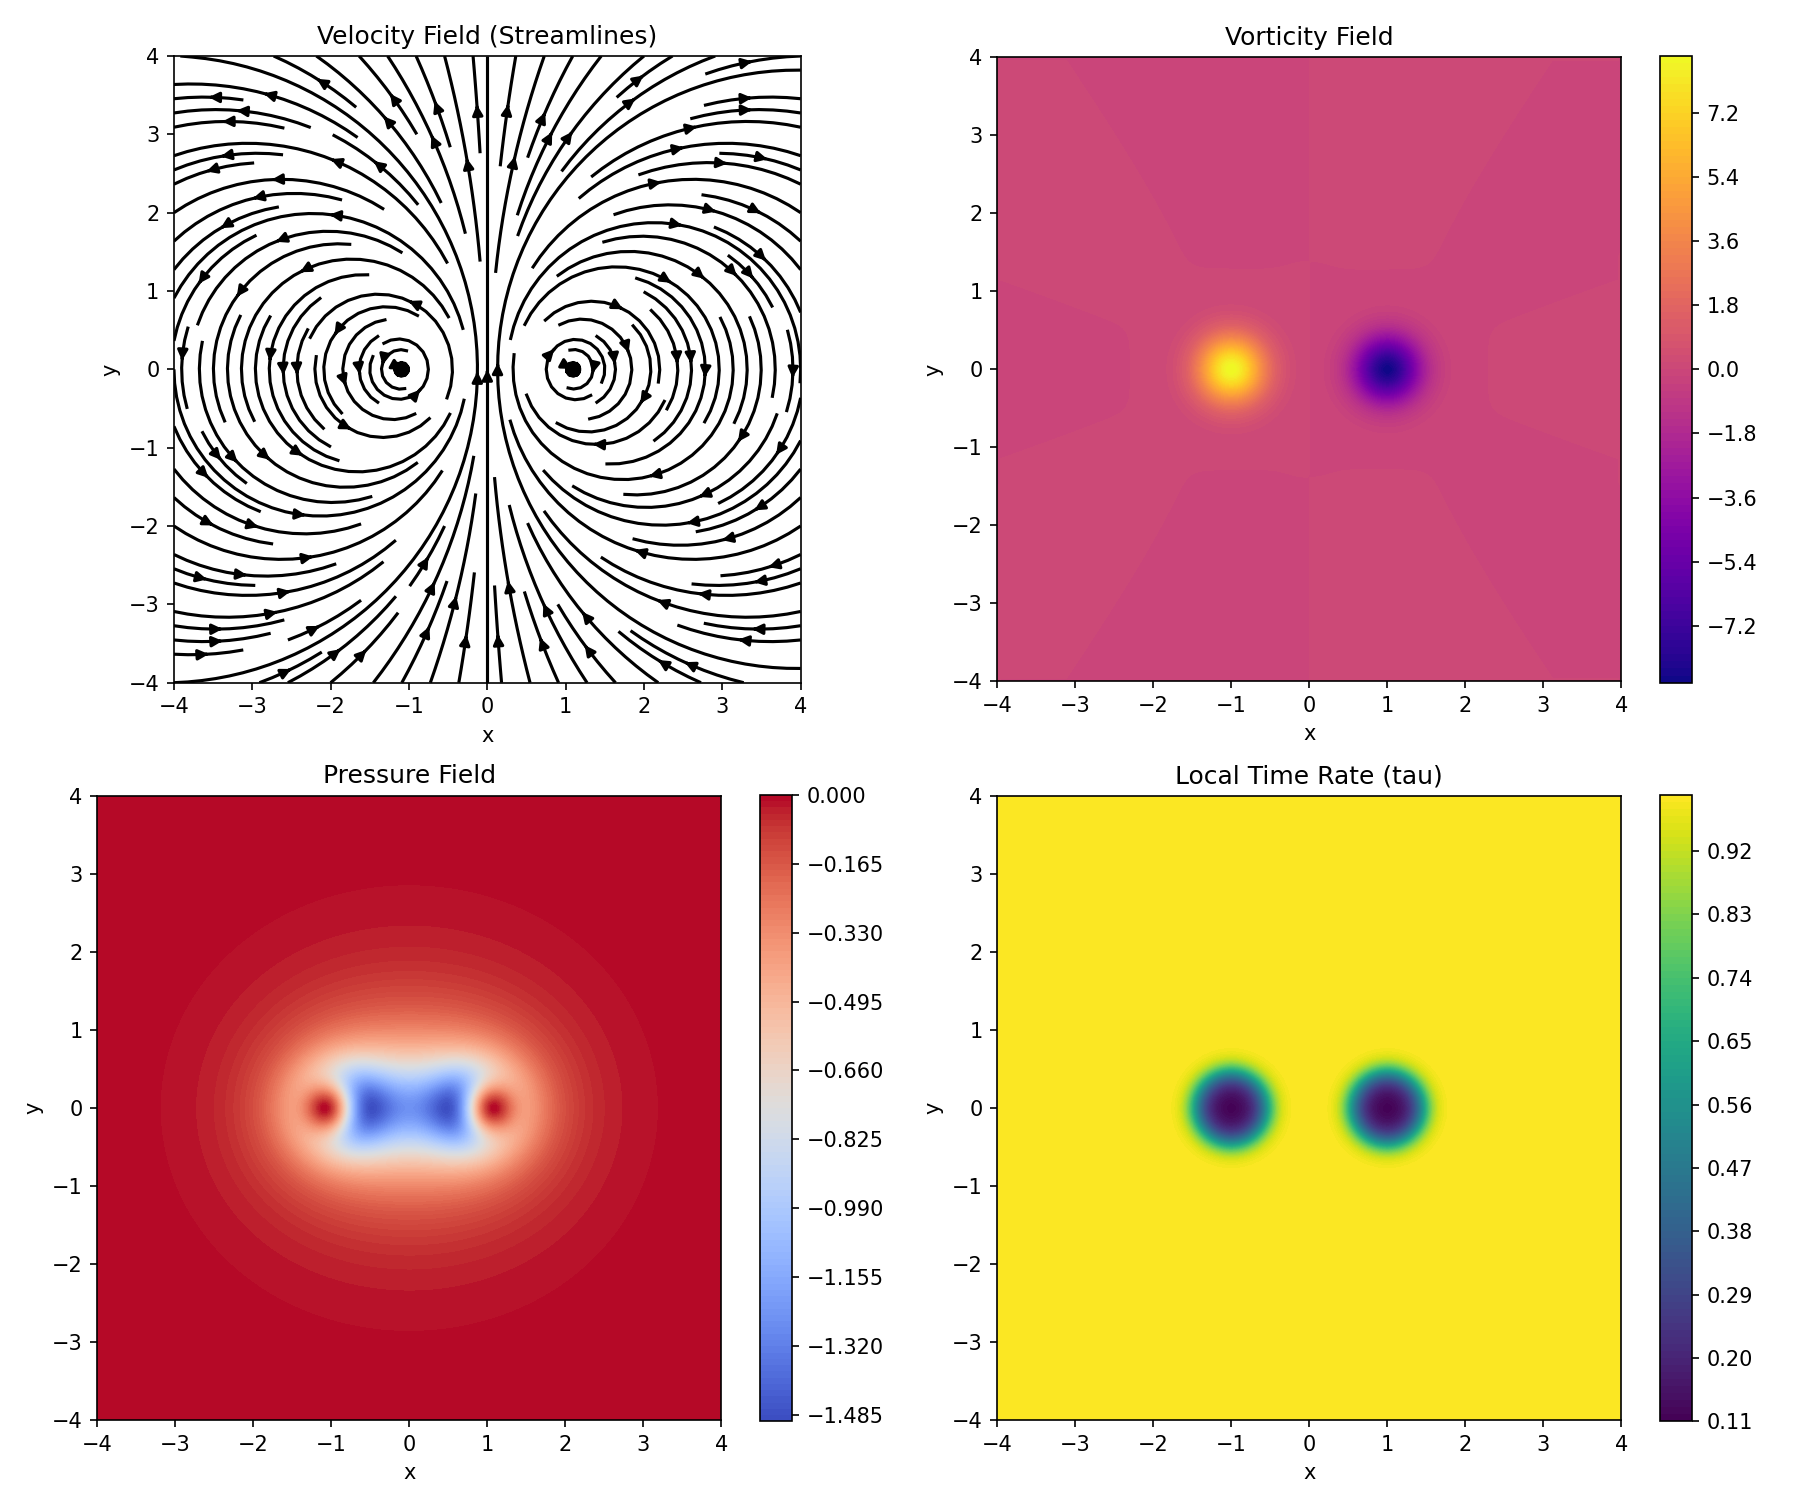
\includegraphics[width=0.85\textwidth]{streamlinesDiPole}
    \caption{Velocity streamlines, vorticity, pressure, and local time rate $\tau$ for a simulated vortex pair. The pressure minimum and time slow-down clearly align with the regions of high vorticity. This directly illustrates the æther model's central claim: time dilation follows from vortex energetics and pressure depletion.}
    \label{fig:vortexfields}
\end{figure}

\subsection{Bernoulli Flow and Local Time Depletion}

In a classical, inviscid, incompressible fluid, Bernoulli's equation describes the conservation of energy in a flow:

\begin{equation}
    \frac{1}{2} \rho_{\text{\ae}}  v^2 + p = p_0 \Rightarrow p = p_0 - \frac{1}{2} \rho_{\text{\ae}} v^2\label{eq:bernoulli}
\end{equation}

Here:
\begin{itemize}
    \item $p_0$ is the background reference pressure,
    \item $\rho_{\text{\ae}}$ is the constant æther density,
    \item $v$ is the local velocity of the æther near the vortex.
\end{itemize}

Assuming that clock rate is proportional to pressure (i.e., time slows in low-pressure regions), we relate the local clock frequency to the background as:

\begin{equation}
    \frac{f_{\text{local}}}{f_0} = 1 - \frac{\rho_{\text{\ae}} v^2}{2 p_0}\label{eq:local_clock_frequency}
\end{equation}

Hence, time dilation is:

\begin{equation}
    \frac{t_{\text{local}}}{t_0} = \left(1 - \frac{\rho_{\text{\ae}} v^2}{2 p_0}\right)^{-1}\label{eq:time_dilation}
\end{equation}

For rotational flow, with $v = \Omega r$,

\begin{equation}
    \frac{t_{\text{local}}}{t_0} = \left(1 - \frac{\rho_{\text{\ae}} \Omega^2 r^2}{2 p_0} \right)^{-1} \approx 1 + \frac{\rho_{\text{\ae}}\Omega^2 r^2}{2 p_0}\label{eq:time_dilation_rotational}
\end{equation}

This expression recovers the first-order time dilation analog if we define the dimensionless coupling:

\begin{equation}
    \frac{\rho_{\text{\ae}}}{p_0} \sim \frac{1}{c^2}\label{eq:dimensionless_coupling}
\end{equation}

This motivates the analogy to relativistic time dilation:

\begin{equation}
    \frac{t_{\text{moving}}}{t_\text{rest}} \approx 1 + \frac{v^2}{2 c^2}\label{eq:relativistic_time_dilation}
\end{equation}

\begin{figure}[htbp]
    \centering
    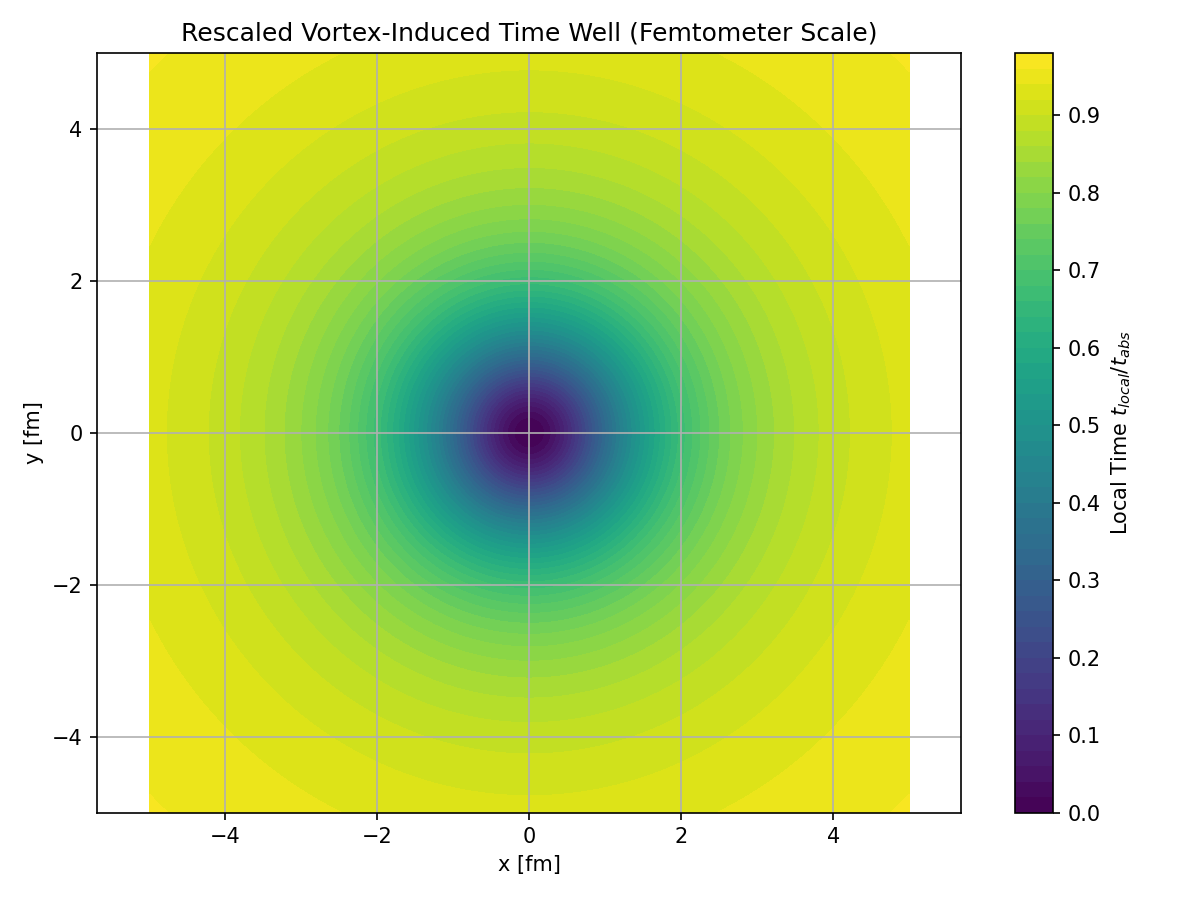
\includegraphics[width=0.8\textwidth]{RadialProfileOfLocalTimeDilation_Vortex-Induced_Time_Well}
    \caption{Schematic of a vortex-induced time well in the æther. Local time $t_{\text{local}} / t_{\text{abs}}$ is shown as a color gradient in 2D space. The central vortex region exhibits the most time slowing due to high $\Omega_k$, forming a well-like structure.}
    \label{fig:vortex_time_well}
\end{figure}


\subsection{Heuristic Knot-Based Time Modulation}

Topological vortex knots have intrinsic angular frequency $\Omega_k$, conserved due to vorticity confinement. We introduce a first-principles motivated
time dilation expression:

\begin{equation}
\frac{t_{\text{local}}}{t_{\text{abs}}} = \left(1 + \alpha \Omega_k^2 \right)^{-1}\label{eq:angular_time_dilation}
\end{equation}

where $\alpha$ is a coupling parameter with dimensions $[\alpha] = \text{s}^2$. Expanding for small $\Omega_k$:

\begin{equation}
\frac{t_{\text{local}}}{t_{\text{abs}}} \approx 1 - \alpha \Omega_k^2 + \mathcal{O}(\Omega_k^4)\label{eq:angular_time_dilation_expansion}
\end{equation}

This form parallels the Lorentz factor expansion:

\begin{equation}
\frac{t_{\text{moving}}}{t_{\text{rest}}} \approx 1 - \frac{v^2}{2 c^2}\label{eq:lorentz_time_dilation}
\end{equation}

\begin{figure}[htbp]
    \centering
    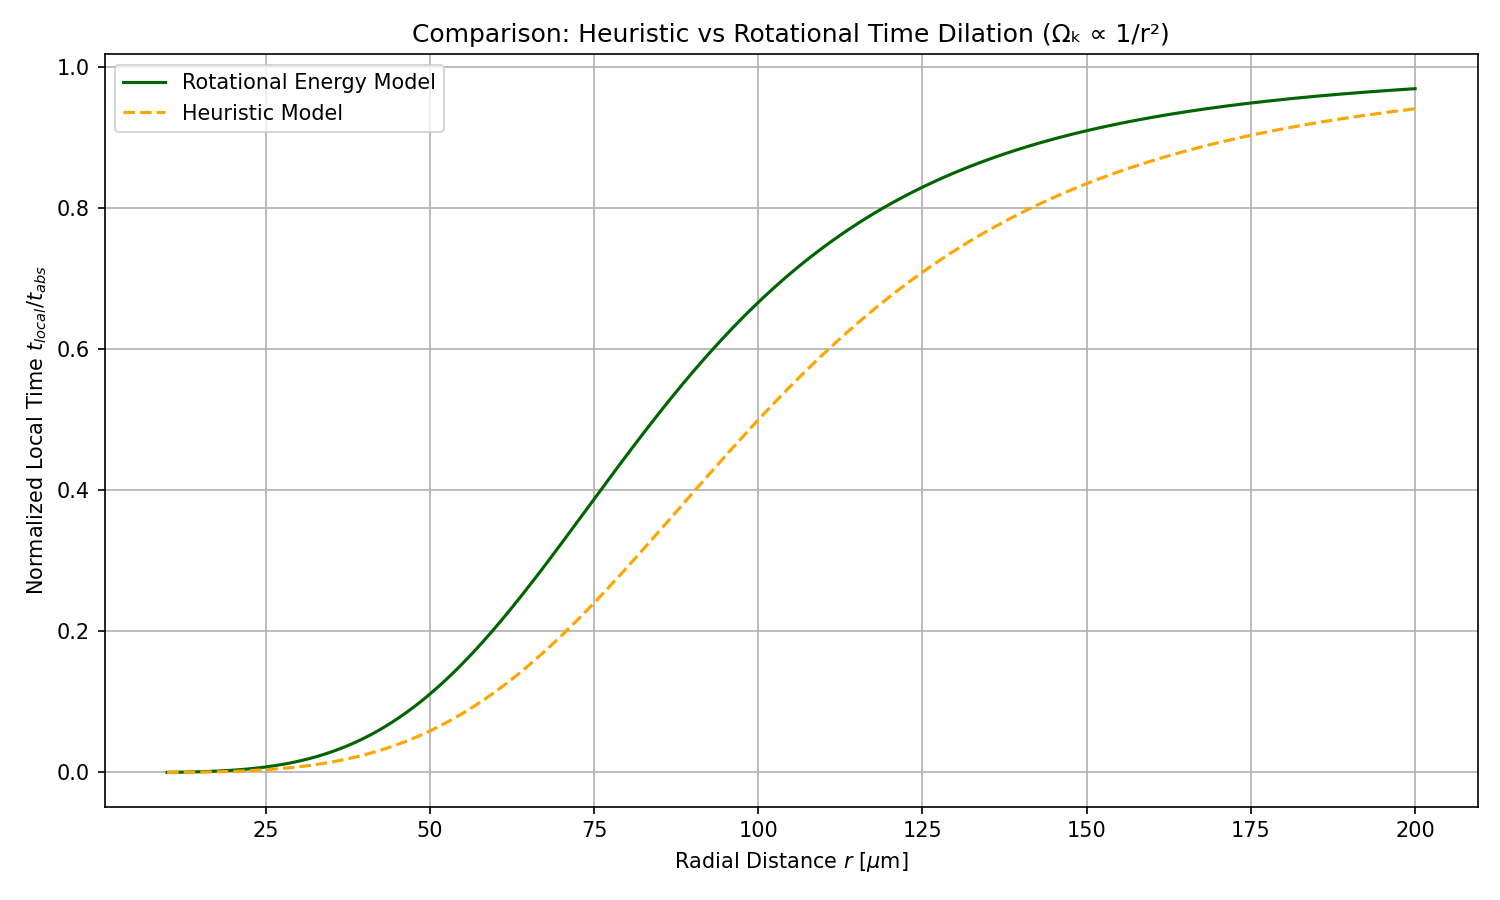
\includegraphics[width=0.8\textwidth]{RotationalVsHeuristicTimeDilation}
    \caption{\textbf{Comparison: Heuristic vs Rotational Time Dilation (\(\Omega_k \propto 1/r^2\))}.
    This graph compares two models of time modulation within the Vortex Æther framework.
    The heuristic model (green) assumes time rate reduction proportional to \((1 + \alpha \Omega_k^2)^{-1}\),
        while the rotational model (dark blue) incorporates rotational energy \(E_{\text{rot}} = \frac{1}{2} I \Omega_k^2\) and suppresses local time via
        \((1 + \frac{1}{2} \alpha I \Omega_k^2)^{-1}\). Both curves exhibit strong time dilation near the vortex core (\(r \sim 10^{-15}\) m),
        approaching absolute time flow only at extended distances. The rotational model yields a steeper suppression,
        highlighting the energetic cost of maintaining high angular momentum in fluid-based time curvature.
    }
    \label{fig:radial_time_profile}
\end{figure}

\subsection{Time Dilation from Rotational Inertia}

We now ground the heuristic form in physical energetics. For a knot with moment of inertia $I$, the rotational energy is:

\begin{equation}
E_{\text{rot}} = \frac{1}{2} I \Omega_k^2\label{eq:rotational_energy}
\end{equation}

Thus, the time dilation becomes:

\begin{equation}
\frac{t_{\text{local}}}{t_{\text{abs}}} = \left(1 + \alpha E_{\text{rot}} \right)^{-1} = \left(1 + \frac{1}{2} \alpha I \Omega_k^2 \right)^{-1}\label{eq:time_dilation_rotational_energy}
\end{equation}

This is the key result:

\begin{equation}
    \boxed{\frac{t_{\text{local}}}{t_{\text{abs}}} = \left(1 + \frac{1}{2} \alpha I \Omega_k^2 \right)^{-1}}
    \label{eq:localtime_vortex}
\end{equation}

\subsection{Summary of Model Hierarchy}

\begin{itemize}
\item Pressure-Based (Bernoulli): Time slows in low-pressure zones due to vortex velocity.
\item Heuristic Angular Model: Time slows proportionally to $\Omega_k^2$.
\item Energetic Model: Time flow depends on stored rotational energy in the knot.
\end{itemize}

These form a continuum of physical justification, culminating in a replacement of spacetime curvature with rotational æther mechanics. This establishes the VAM time dilation framework as a fluidic, topologically-conserved analog to GR.

Next, we will explore how these models correspond to GR-like metrics and rotational observers in Section II.
\section{Entropy and Quantum Effects in the Vortex Æther Model}

The Vortex Æther Model (VAM) provides a mechanistic basis for both thermodynamic and quantum mechanical phenomena, not through postulates about abstract state spaces, but via the dynamics of knots and vortices in a superfluid æther. Two central concepts—entropy and quantization—are derived in VAM from vorticity distribution and knot topology, respectively.

\subsection{Entropy as vorticity distribution}

In thermodynamics, entropy $S$ is a measure of the internal energy distribution or disorder. In VAM, entropy does not arise as a statistical phenomenon, but from spatial variations in vorticity. For a vortex configuration $V$ the entropy is given by:

\begin{equation}
    S \propto \int_V \|\vec{\omega}\|^2 \, dV,
\end{equation}

where $\vec{\omega} = \nabla \times \vec{v}$ is the local vorticity. This means:

\begin{itemize}
    \item \textbf{More rotation = more entropy}: Regions with strong swirl contribute to increased entropy.
    \item \textbf{Thermodynamic behavior arises from vortex expansion}: With the addition of energy (heat), the vortex boundary expands, the swirl decreases and $S$ increases—analogy with gas expansion.
\end{itemize}

This interpretation connects Clausius' heat theory with æther mechanics: heat is equivalent to increased swirl spreading.

\subsection{Quantum behavior from knotted vortex structures}

Quantum phenomena such as discrete energy levels, spin, and wave-particle duality originate in VAM from topologically conserved vortex knots:

\begin{itemize}
    \item \textbf{Circulation quantization:}
    \begin{equation}
        \Gamma = \oint \vec{v} \cdot d\vec{l} = n \cdot \kappa,
    \end{equation}
    where $\kappa = h/m$ and $n \in \mathbb{Z}$ is the winding number.
    \item \textbf{Integers arise from knot topology:} The helical structure of a vortex knot (such as a trefoil) provides discrete states with certain linking numbers $L_k$.
    \item \textbf{Helicity as a spin analogue:}
    \begin{equation}
        H = \int \vec{v} \cdot \vec{\omega} \, dV,
    \end{equation}
    where $H$ is invariant under ideal flow, just as spin is conserved in quantum mechanics.
\end{itemize}

\subsection{VAM interpretation of quantization and duality}

Instead of abstract Hilbert spaces, VAM considers a particle as a stable node in the æther field. This vortex configuration has:

\begin{itemize}
    \item A \textbf{core} (nodal body) with quantum jumps (resonances).
    \item An \textbf{outer field} that acts as a wave (like the Schrödinger wave).

    \item A \textbf{helicity} that behaves as internal degrees of freedom (e.g. spin).
\end{itemize}

The wave-particle dualism thus arises from the fact that knots are both localized (core) and spread out (field).

\subsection{Summary}

VAM thus provides a coherent, fluid-mechanical origin for both:

\begin{enumerate}
    \item \textbf{Thermodynamics:} Entropy arises from swirl distribution.
    \item \textbf{Quantum mechanics:} Quantization and duality are emergent properties of knotted vortex topologies.
\end{enumerate}

This approach shows that quantum and thermodynamic phenomena are not fundamentally different, but arise from the same vortex mechanism at different scales.

\section*{Entropy as a Vorticity-Weighted Invariant}\label{sec:entropy_vorticity}

In the Vortex Æther Model (VAM), we reinterpret classical entropy as a conserved scalar related to the internal vorticity structure of knotted field regions. The classical thermodynamic differential form:
\begin{equation}
    dS = \frac{\delta Q}{T},
\end{equation}
acquires a new form when heat exchange is replaced by rotational stress input into vortex knots:
\begin{equation}
    dS = \frac{\delta \Pi_\text{rot}}{\mathcal{T}_\omega},
\end{equation}
where:
\begin{itemize}
    \item $\delta \Pi_\text{rot}$ is the differential rotational energy input to the vortex core,
    \item $\mathcal{T}_\omega$ is the effective swirl-defined temperature field,
    \item $\omega = \nabla \times \vec{v}$ is the local vorticity.
\end{itemize}
This connects thermodynamic irreversibility directly to vorticity injection and local time dilation.

\subsection*{VAM Pressure Gradients and Entropy Flow}

In VAM, pressure gradients are induced by angular momentum conservation in the æther. The classical Euler equation for incompressible inviscid flow:
\begin{equation}
    \nabla P = -\rho_\text{\ae} (\vec{v} \cdot \nabla) \vec{v},
\end{equation}
is used to express entropy production through vorticity current divergence:
\begin{equation}
    \frac{dS}{dt} = \int_V \frac{\nabla \cdot \vec{J}_\text{vortex}}{T_\omega} \, dV,
\end{equation}
where $\vec{J}_\text{vortex}$ is the swirl energy flux density. This forms the entropy production analogue of Fourier's heat conduction law within the vortex medium.

\subsection*{Thermal Expansion of Vortex Knots}

Inspired by Clausius' treatment of thermal expansion, we define a vorticity-based expansion law for knotted vortex structures:
\begin{equation}
    \Delta V_\text{knot} = \alpha_\omega V_0 \Delta T_\omega,
\end{equation}
with:
\begin{equation}
    \alpha_\omega = \frac{1}{r_c} \frac{d r_k}{d T_\omega} \sim \frac{C_e^2}{r_c k_B T_\omega},
\end{equation}
where $r_k$ is the effective knot radius, $r_c$ is the core radius, $C_e$ the core swirl velocity, and $k_B$ the Boltzmann constant. Knot inflation in VAM thus follows from ætheric heating.

\subsection*{Clausius Inequality and Helicity Dissipation}

The Clausius inequality:
\begin{equation}
    \oint \frac{\delta Q}{T} \leq 0,
\end{equation}
is reinterpreted in VAM as a constraint on helicity-induced vorticity flow:
\begin{equation}
    \oint \frac{\vec{v} \cdot d\vec{\omega}}{\mathcal{T}_\omega} \leq 0,
\end{equation}
which implies that net swirl energy circulation around closed loops is dissipative unless compensated by external ætheric drive. This underpins the irreversibility of vortex-knot interactions.

\subsection*{Carnot Efficiency in Swirl Fields}

Classical Carnot engine efficiency:
\begin{equation}
    \eta = 1 - \frac{T_C}{T_H},
\end{equation}
can be reformulated in VAM via vorticity amplitudes:
\begin{equation}
    \eta_\text{VAM} = 1 - \frac{\Omega_C^2}{\Omega_H^2},
\end{equation}
where $\Omega_H$ and $\Omega_C$ are internal angular velocities of vortex knots in high and low swirl zones. This formulation links macroscopic energy conversion directly to microscopic vorticity gradients.


\section{Time modulation by rotation of vortex nodes}

Building on the discussion of time dilation via pressure and Bernoulli dynamics in the previous section, we now focus on the intrinsic rotation of topological vortex nodes. In the Vortex Æther Model (VAM), particles are modeled as stable, topologically conserved vortex nodes embedded in an incompressible, inviscid superfluid medium. Each node possesses a characteristic internal angular frequency $\Omega_k$, and this internal motion induces local time modulation with respect to the absolute time of the æther.

Instead of warping spacetime, we propose that internal rotational energy and helicity conservation cause temporal delays analogous to gravitational redshift. In this section, these ideas are developed using heuristic and energetic arguments consistent with the hierarchy introduced in Section I.

\subsection{Heuristic and energetic derivation}

We start by proposing a rotational induced time dilation formula based on the internal angular frequency of the node:

\begin{equation}
    \frac{t_\text{local}}{t_\text{abs}} = \left(1 + \beta \Omega_k^2 \right)^{-1}\label{eq:rotational_induced_time_dilation}
\end{equation}

where:

\begin{itemize}
    \item $t_\text{local}$ is the proper time near the node,
    \item $t_\text{abs}$ is the absolute time of the background æther,
    \item $\Omega_k$ is the mean core angular frequency,
    \item $\beta$ is a coupling coefficient with dimensions $[\beta] = \text{s}^2$.
\end{itemize}

For small angular velocities we obtain a first-order expansion:

\begin{equation}
    \frac{t_\text{local}}{t_\text{abs}} \approx 1 - \beta \Omega_k^2 + \mathcal{O}(\Omega_k^4)\label{eq:rotational_induced_time_dilation_expansion}
\end{equation}

This form parallels the Lorentz factor at low velocities in special relativity:

\begin{equation}
    \frac{t_\text{moving}}{t_\text{rest}} \approx 1 - \frac{v^2}{2c^2}\label{eq:parallels_lorentz_time_dilation}
\end{equation}

This yields a important analogy: Internal rotational motion in VAM induces time dilation, similar to how translational velocity induces time dilation in SR.

To strengthen the physical basis of this expression, we now relate time dilation to the energy stored in vortex rotation. Suppose the vortex node has an effective moment of inertia $I$. The rotational energy is given by:

\begin{equation}
    E_\text{rot} = \frac{1}{2} I \Omega_k^2\label{eq:rotational_energy_inertia}
\end{equation}

Assuming that time slows down due to this energy density, we write:

\begin{equation}
    \frac{t_\text{local}}{t_\text{abs}} = \left(1 + \beta E_\text{rot} \right)^{-1} = \left(1 + \frac{1}{2} \beta I \Omega_k^2 \right)^{-1}\label{eq:time_dilation_rotational_energy_inertia}
\end{equation}

This expression serves as the energetic analogue of the pressure-based Bernoulli model from Section I (cf. ~\eqref{eq:vortex_time_dilation}). It supports the interpretation of vortex-induced time wells via energy storage rather than geometric deformation.

\subsection{Topological and physical justification}

Topological vortex nodes are characterized not only by rotation, but also by helicity:

\begin{equation}
    H = \int \vec{v} \cdot \vec{\omega} \, d^3x \label{eq:helicity_rotation}
\end{equation}

Helicity is a conserved quantity in ideal (invisible, incompressible) fluids, which encodes the connection and rotation of vortex lines. The rotation frequency $\Omega_k$ becomes a topologically meaningful indicator of the identity and dynamic state of the node.

Higher $\Omega_k$ values indicate more rotational energy and deeper pressure wells, leading to transient delays that resemble gravitational redshift, but without spacetime curvature.

Each particle is a topological vortex knot:
\begin{itemize}
    \item Charge $\leftrightarrow$ rotation or chirality of the knot
    \item Mass $\leftrightarrow$ integrated vorticity energy
    \item Spin $\leftrightarrow$ knot helix:
\end{itemize}
Stability $\leftrightarrow$ knot type (Hopf connections, Trefoil, etc.) and energy minimization in the vortex core

This model:

\begin{itemize}
    \item Attributes time modulation to conserved, intrinsic rotational energy,
    \item Requires no external frames of reference (absolute æther time is universal),
    \item Preserves temporal isotropy outside the vortex core,
    \item Provides a natural replacement for the spacetime curvature of GR. \end{itemize}

Therefore, this vortex-energetic time dilation principle provides a powerful alternative to relativistic time modulation by anchoring all temporal effects in rotational energetics and topological invariants.

In the next section, we will show how these ideas reproduce metric-like behavior for rotating observers, including a direct fluid-mechanical analogue to the Kerr metric of general relativity.
\input{Swirl_Clocks/03_Proper_Time_for_a_Rotating_Observer_in_Æther_Flow}
\section{Kerr-like time adjustment based on vorticity and circulation}

To complete the analogy between general relativity (GR) and the vortex-æther model (VAM), we now derive a time modulation formula that reflects the redshift and frame-dragging structure in the Kerr solution. In GR, the Kerr metric describes the spacetime geometry around a rotating mass and predicts both gravitational time dilation and frame-dragging due to angular momentum. VAM captures similar phenomena via the dynamics of structured vorticity and circulation in the æther, without the need for spacetime curvature.

\subsection{General relativistic Kerr redshift structure}

In the GR-Kerr metric, the proper time $d\tau$ for an observer near a rotating mass is affected by both mass-energy and angular momentum. A simplified approximation for the time dilation factor near a rotating body is:
\begin{equation}
    t_{\text{adjusted}} = \Delta t \cdot \sqrt{1 - \frac{2GM}{rc^2} - \frac{J^2}{r^3c^2}}
    \label{eq:Kerr_time_dilation}
\end{equation}
where:
\begin{itemize}
    \item $M$: mass of the rotating body,
    \item $J$: angular momentum,
    \item $r$: radial distance from the source,
    \item $G$: Newton's gravitational constant,
    \item $c$: speed of light.
\end{itemize}

The first term corresponds to gravitational redshift with respect to the mass, while the second takes into account rotational effects (frame-dragging).

\subsection{Æther analogous via vorticity and circulation}

In VAM we express gravitational influences via vorticity intensity $\langle \omega^2 \rangle$ and total circulation $\kappa$. These are interpreted as:
\begin{itemize}
    \item $\langle \omega^2 \rangle$: mean square vorticity over a region,
    \item $\kappa$: conserved circulation, encoding angular momentum.

\end{itemize}

We define the æther-based analogue by performing the following replacements:
\begin{equation}
    \begin{aligned}
        \frac{2GM}{rc^2} &\rightarrow \frac{\gamma \langle \omega^2 \rangle}{rc^2}, \\
        \frac{J^2}{r^3c^2} &\rightarrow \frac{\kappa^2}{r^3c^2}
    \end{aligned}
    \label{eq:Kerr_replacements}
\end{equation}

Here $\gamma$ is a coupling constant relating the vorticity to the effective gravity (analogous to $G$). The æther-based proper then becomes:

\begin{equation}
    \boxed{t_{\text{adjusted}} = \Delta t \cdot \sqrt{1 - \frac{\gamma \langle \omega^2 \rangle}{rc^2} - \frac{\kappa^2}{r^3c^2}}}
    \label{eq:Kerr_time_dilation_ae}
\end{equation}

This reflects the Kerr redshift and frame dragging structure using fluid dynamic variables. In this figure:
\begin{itemize}
    \item $\langle \omega^2 \rangle$ plays the role of energy density that produces gravitational redshift,
    \item $\kappa$ represents angular momentum that generates temporal frame-dragging,
    \item The equation reduces to a flat æther time ($t_{\text{adjusted}} \tot \Delta t$) when both terms vanish.

\end{itemize}

\subsection*{Hybrid VAM Frame-Dragging Angular Velocity}

In the Vortex Æther Model (VAM), the frame-dragging angular velocity induced by a rotating vortex-bound object is defined analogously to the Lense-Thirring effect in general relativity, but with a scale-dependent Coupling:

\begin{equation}
    \omega_{\text{drag}}^{\text{VAM}}(r) =
    \frac{4 G m}{5 c^2 r} \cdot \mu(r) \cdot \Omega(r)
\end{equation}

Where \( G \) is the gravitational constant, \( c \) is the speed of light, \( m \) is the mass of the object, \( r \) is the characteristic radius, and \( \Omega(r) \) the angular velocity.

The hybrid coupling factor \( \mu(r) \) interpolates between quantum-scale vortex behavior and classical macroscopic rotation:

\begin{equation}
    \mu(r) =
    \begin{cases}
        \displaystyle \frac{r_c C_e}{r^2}, & \text{if } r < r_\ast \quad \text{(quantum or vortex core regime)} \\
        1, & \text{if } r \geq r_\ast \quad \text{(macroscopic regime)}
    \end{cases}
\end{equation}

where:
\begin{itemize}
    \item \( r_c \) is the radius of the vortex core,
    \item \( C_e \) is the tangential velocity of the vortex core,
    \item \( r_\ast \sim 10^{-3} \, \text{m} \) is the transition radius between microscopic and macroscopic regimes.
\end{itemize}

This formulation provides continuity with GR predictions for celestial bodies, while allowing VAM-specific predictions for elementary particles and subatomic vortex structures.

\subsection*{VAM Gravitational Redshift from Core Rotation}

In the Vortex Æther Model (VAM), gravitational redshift arises from the local rotation velocity \( v_\phi \) at the outer boundary of a vortex node. Assuming no spacetime curvature and absolute time, the effective gravitational redshift is given by:

\begin{equation}
    z_{\text{VAM}} =
    \left( 1 - \frac{v_\phi^2}{c^2} \right)^{-\frac{1}{2}} - 1
\end{equation}

where:
\begin{itemize}
    \item \( v_\phi = \Omega(r) \cdot r \) is the tangential velocity due to local rotation,
    \item \( \Omega(r) \) is the angular velocity at the measurement beam \( r \),
    \item \( c \) is the speed of light in vacuum.

\end{itemize}

This expression reflects the change in time perception caused by local rotational energy, replacing the curvature-based gravitational potential \( \Phi \) of general relativity with a velocity field term. It becomes equivalent to the GR Schwarzschild redshift for low \( v_\phi \) and diverges as \( v_\phi \rightarrow c \), which provides a natural limit to the evolution of the local frame:

\begin{equation}
    \lim_{v_\phi \to c} z_{\text{VAM}} \to \infty
\end{equation}

\subsection*{VAM Local Time Dilation Models}

In the Vortex Æther Model (VAM), local time dilation is interpreted as the modulation of absolute time by internal vortex dynamics, not by spacetime curvature. Depending on the system scale, two physically based formulations are used:

\paragraph{1. Time dilation based on velocity fields}

This model relates the local time flow to the tangential speed of the rotating etheric structure (vortex node, planet or star):

\begin{equation}
    \frac{d\tau}{dt} =
    \sqrt{1 - \frac{v_\phi^2}{c^2}} =
    \sqrt{1 - \frac{\Omega^2 r^2}{c^2}}
\end{equation}

whereby:
\begin{itemize}
    \item \( v_\phi = \Omega \cdot r \) is the tangential speed,
    \item \( \Omega \) is the angular velocity at radius \( r \),
    \item \( c \) is the speed of light.
\end{itemize}

\paragraph{2. Time dilation based on rotational energy}

On large scales or with high rotational inertia, time dilation arises from stored rotational energy, leading to:

\begin{equation}
    \frac{d\tau}{dt} =
    \left(1 + \frac{1}{2} \cdot \beta \cdot I \cdot \Omega^2 \right)^{-1}
\end{equation}

with:
\begin{itemize}
    \item \( I = \frac{2}{5} m r^2 \): moment of inertia for a uniform sphere,
    \item \( \beta = \frac{r_c^2}{C_e^2} \): coupling constant of vortex-core dynamics,
    \item \( m \) is the mass of the object. \end{itemize}

\paragraph{Interpretation}

These models imply that time slows down in regions of high local rotational energy or vorticity, consistent with gravitational time dilation effects in GR. In VAM, however, these effects arise exclusively from the internal dynamics of the æther flow, under flat 3D Euclidean geometry and absolute time.

\subsection{Model assumptions and scope}

This result depends on several assumptions:
\begin{itemize}
    \item The flow is irrotational outside the vortex cores,
    \item Viscosity and turbulence are neglected,
    \item Compressibility is ignored (ideal incompressible superfluid),
    \item Vorticity fields are sufficiently smooth to define $\langle \omega^2 \rangle$.
\end{itemize}

These conditions reflect the assumptions of analogous models of ideal fluid GR. The formulation bridges the macroscopic fluid dynamics of the æther with effective geometric predictions, which strengthens the possibility of replacing curved spacetime with structured vorticity fields.

See Appendix~\ref{appendix:7} for detailed derivations of cross-energy and vortex interaction energetics.

In future work, corrections for boundary conditions, quantized vorticity spectra, and compressibility effects can be added to refine the analogy. We then summarize how these fluid-based time dilation mechanisms coalesce within the VAM framework and identify their experimental implications.
\section{Unified Framework and Synthesis of Time Dilation in VAM}

This section unifies the time dilation mechanisms discussed in the paper under the Vortex Æther Model (VAM). Instead of relying on spacetime curvature, VAM attributes temporal effects to classical fluid dynamics, rotational energy, and topological vorticity.

\subsection{Hierarchical Structure of Time Dilation Mechanisms}

Each section of this work contributes a separate but interrelated mechanism for time dilation:

\begin{enumerate}
    \item \textbf{Bernoulli-Induced Time Depletion:} Time slows down near regions of low pressure due to vortex-induced kinetic velocity fields. This results in a special relativistic time dilation form when \( \rho_{\text{\ae}} / p_0 \sim 1/c^2 \).
    \item \textbf{Heuristic model for angular frequency:} A quadratic dependence of the time velocity on the local nodal angular frequency \( \Omega_k^2 \), which mimics the Lorentz factor expansion for small velocities.
    \item \textbf{Energetic formulation via rotational inertia:}
    \[
        \boxed{\frac{t_{\text{local}}}{t_{\text{abs}}} = \left(1 + \frac{1}{2} \beta I \Omega_k^2 \right)^{-1}}
    \]
    directly links time modulation to the rotational energy of vortex nodes. \item \textbf{Own time stream based on velocity field:}
    \[
        \boxed{\left( \frac{d\tau}{dt} \right)^2 = 1 - \frac{1}{c^2}(v_r + r\Omega_k)^2}
    \]
    \item \textbf{Kerr-like redshift and frame drag:}
    \[
        \boxed{t_{\text{adjusted}} = \Delta t \cdot \sqrt{1 - \frac{\gamma \langle \omega^2 \rangle}{rc^2} - \frac{\kappa^2}{r^3c^2}}}
    \]
\end{enumerate}

These five expressions form a self-consistent ladder, ranging from heuristic to rigorous, and provide a robust replacement for general relativistic time dilation, based entirely on classical field variables.

\subsection{Physical unification: Time as a vorticity-derived observable}

A recurring theme emerges in all formulations: \textit{time modulation in VAM is always reducible to local kinetic or rotational energy density within the æther}. Whether encoded in pressure (Bernoulli), angular frequency (\( \Omega_k \)) or field circulation (\( \kappa \)), the modulation of time is not geometric but energetic and topological.

\begin{itemize}
    \item Local time wells arise from high vorticity and circulation.
    \item Frame independence: Absolute time exists; only local velocities are affected.
    \item No need for tensor geometry: All time effects arise from scalar or vector fields.
    Topological conservation: Vortices preserve helicity and circulation, which provides temporal consistency.

    This unification strengthens the conceptual core of VAM: spacetime curvature is an emergent illusion caused by structured vorticity in an absolute, superfluid æther.

    Experimental implications and prospects

    Each time dilation formula introduced here can in principle be tested in analogous laboratory systems:

    Rotating superfluid droplets (e.g., helium-II, BECs)
    Electrohydrodynamic lifters and plasma vortex systems
    Magnetofluidic and optical analogs

    Future work includes:
    Establishment of items
    Deriving dynamical equations for temporal feedback in multi-node systems. \item Measuring vortex-induced clock drift in rotating superfluids.

    \item Applying the model to astrophysical observations (e.g., neutron star precession, frame dragging, time dilation).
\end{itemize}

\subsection{Challenges, limitations, and paths to broader relevance}

\textbf{Fundamental assumptions:} Reintroducing an æther with absolute time poses a challenge to a century of relativistic physics.

\textbf{Experimental validation:} There is no direct empirical evidence yet to support the proposed æther or specific dilation mechanisms.

\textbf{Reception in mainstream physics:} While niche communities may engage, mainstream physics may resist because of deviations from established frameworks.

\subsection{Enhancing scientific rigor and broader appeal}

\begin{itemize}
    \item \textbf{Propose testable predictions:} especially where VAM deviates from GR.
    \item \textbf{Integrate with established theories:} show borderline cases that match GR/QM. \item \textbf{Address historical objections:} clearly redefine æther with modern restrictions.
    \item \textbf{Peer Review and Collaboration:} invite criticism from specialists.
    \item \textbf{Clarity and Accessibility:} simplify the conceptual presentation without sacrificing precision.
\end{itemize}

\subsection{Concluding Perspective}

The Vortex Æther Model (VAM) offers a bold reinterpretation of gravitational time dilation due to vorticity-driven energetics in an absolute, superfluid medium. Through a hierarchy of derivations—encompassing Bernoulli flows, vortex rotation, energy density, and circulation—it provides a coherent alternative to relativistic, curvature-based descriptions. Although VAM departs from conventional theories, its internal logic and conceptual clarity warrant further investigation. Continued refinement, integration, and empirical testing will determine what role the technology will play in further deepening our understanding of gravity, time, and the structure of the universe.
\section{Applications of VAM to quantum and nuclear processes}
\label{sec:LENR_QED}
\subsection*{LENR via resonance tunneling}

Gravitational decay due to vorticity temporarily lowers the Coulomb barrier:

\begin{equation}
    V_\text{Coulomb} = \frac{Z_1 Z_2 e^2}{4\pi \varepsilon_0 r}, \quad \Delta P = \frac{1}{2} \rho_\text{\ae} r_c^2 (\Omega_1^2 + \Omega_2^2)
\end{equation}

Resonance occurs when:

\begin{equation}
    \Delta P \geq \frac{Z_1 Z_2 e^2}{4\pi \varepsilon_0 r_t^2}
\end{equation}

Rather than invoking purely probabilistic tunneling, VAM attributes the transition to real pressure gradients in a structured æther, paralleling the causal flow picture of Holland~\cite{holland1993quantum}

\subsection*{Resonant Ætheric tunneling and LENR in VAM}

In the Vortex Æther Model (VAM), low-energy nuclear reactions (LENR) are reinterpreted as resonant tunneling events mediated by structured vortex interactions in the Æther. Unlike conventional quantum tunneling, which relies on particle wave functions penetrating a static Coulomb potential barrier, VAM posits that local pressure minima – arising from vortex-induced Bernoulli deficits – can temporarily reduce or completely eliminate the barrier~\cite{Barcelo2011,Volovik2003}.

The classical Coulomb repulsion between two nuclei of charges \( Z_1 e \) and \( Z_2 e \) is given by:
\begin{equation}
    V_\text{Coulomb}(r) = \frac{Z_1 Z_2 e^2}{4\pi \varepsilon_0 r}
\end{equation}

In VAM, two rotating vortex nodes in the vicinity of \( r \sim 2r_c \) generate a vortex-induced pressure drop~\cite{Saffman1992} via:
\begin{equation}
    \Delta P = \frac{1}{2} \rho_\text{\ae} r_c^2 (\Omega_1^2 + \Omega_2^2)
\end{equation}

This pressure drop changes the effective interaction potential:
\begin{equation}
    V_\text{eff}(r) = V_\text{Coulomb}(r) - \Phi_\omega(r)
\end{equation}
where the eddy potential \( \Phi_\omega(r) \) is defined by:
\begin{equation}
    \Phi_\omega(r) = \gamma \int \frac{|\vec{\omega}(r')|^2}{|\vec{r} - \vec{r}'|} \, d^3r',
    \quad \text{with} \quad
    \gamma = G \rho_\text{\ae}^2
\end{equation}

Resonant tunneling occurs when the combined effect of \( \Delta P \) and \( \Phi_\omega \) neutralizes the Coulomb barrier at a critical separation \( r_t \):
\begin{equation}
    \frac{1}{2} \rho_\text{\ae} r_c^2 (\Omega_1^2 + \Omega_2^2) \geq \frac{Z_1 Z_2 e^2}{4\pi \varepsilon_0 r_t^2}
\end{equation}

The resulting condition allows for transitions even at thermal or subthermal kinetic energies, allowing LENR processes to occur without actually having to overcome the barrier. Instead, it is dynamically erased via eddy resonance – a mechanism consistent with some empirical observations~\cite{Storms2021}. The tunneling is thus a manifestation of ætheric phase alignment and pressure-mediated coherence in confined vortex configurations.

\subsection*{VAM Quantum Electrodynamics (QED) Lagrangian}

In the Vortex Æther Model (VAM), the interaction between vortex nodes and electromagnetic fields arises from their helical structure and the associated induced vector potentials. The standard Lagrangian of quantum electrodynamics (QED) is replaced in this model by:

\begin{equation}
    \mathcal{L}_\text{VAM-QED} =
    \bar{\psi} \left[ i \gamma^\mu \partial_\mu
                   - \gamma^\mu \left( \frac{C_e^2 r_c}{\lambda_c} \right) A_\mu
                   - \left( \frac{8\pi \rho_\text{\ae} r_c^3 Lk}{C_e} \right) \right] \psi
    - \frac{1}{4} F_{\mu\nu} F^{\mu\nu}
\end{equation}

In this formulation:

\begin{itemize}
    \item Does the mass arise as a result of topological connected vortex cores, where the helicity of the vortex structure plays the role of mass~\cite{Volovik2003}.
    \item The gauge coupling arises from æther circulation and the resulting vector potential.
    \item The electromagnetic field tensor \( F_{\mu\nu} \) remains unchanged, which describes the rotation of the æther (the curl component) in the surrounding superfluid.
\end{itemize}

This alternative Lagrangian thus directly couples vortex structures to field interactions, where the usual constants \( m \) (mass) and \( q \) (charge) are replaced by emergent terms arising from the geometry, rotation rate and topology of the æther medium.

By deriving the Euler–Lagrange equation for the spinor field \( \psi \), we find:

\begin{equation}
    \boxed{ \left( i \gamma^\mu \partial_\mu - \gamma^\mu q_\text{vortex} A_\mu - M_\text{vortex} \right)\psi = 0 }
\end{equation}

This equation is structurally identical to the Dirac equation, but with physical parameters arising from vortex mechanics instead of as fundamental data. Thus, VAM provides an alternative for the origin of mass and charge~\cite{Barcelo2011,Volovik2003}.

\begin{figure}[H]
    \centering
    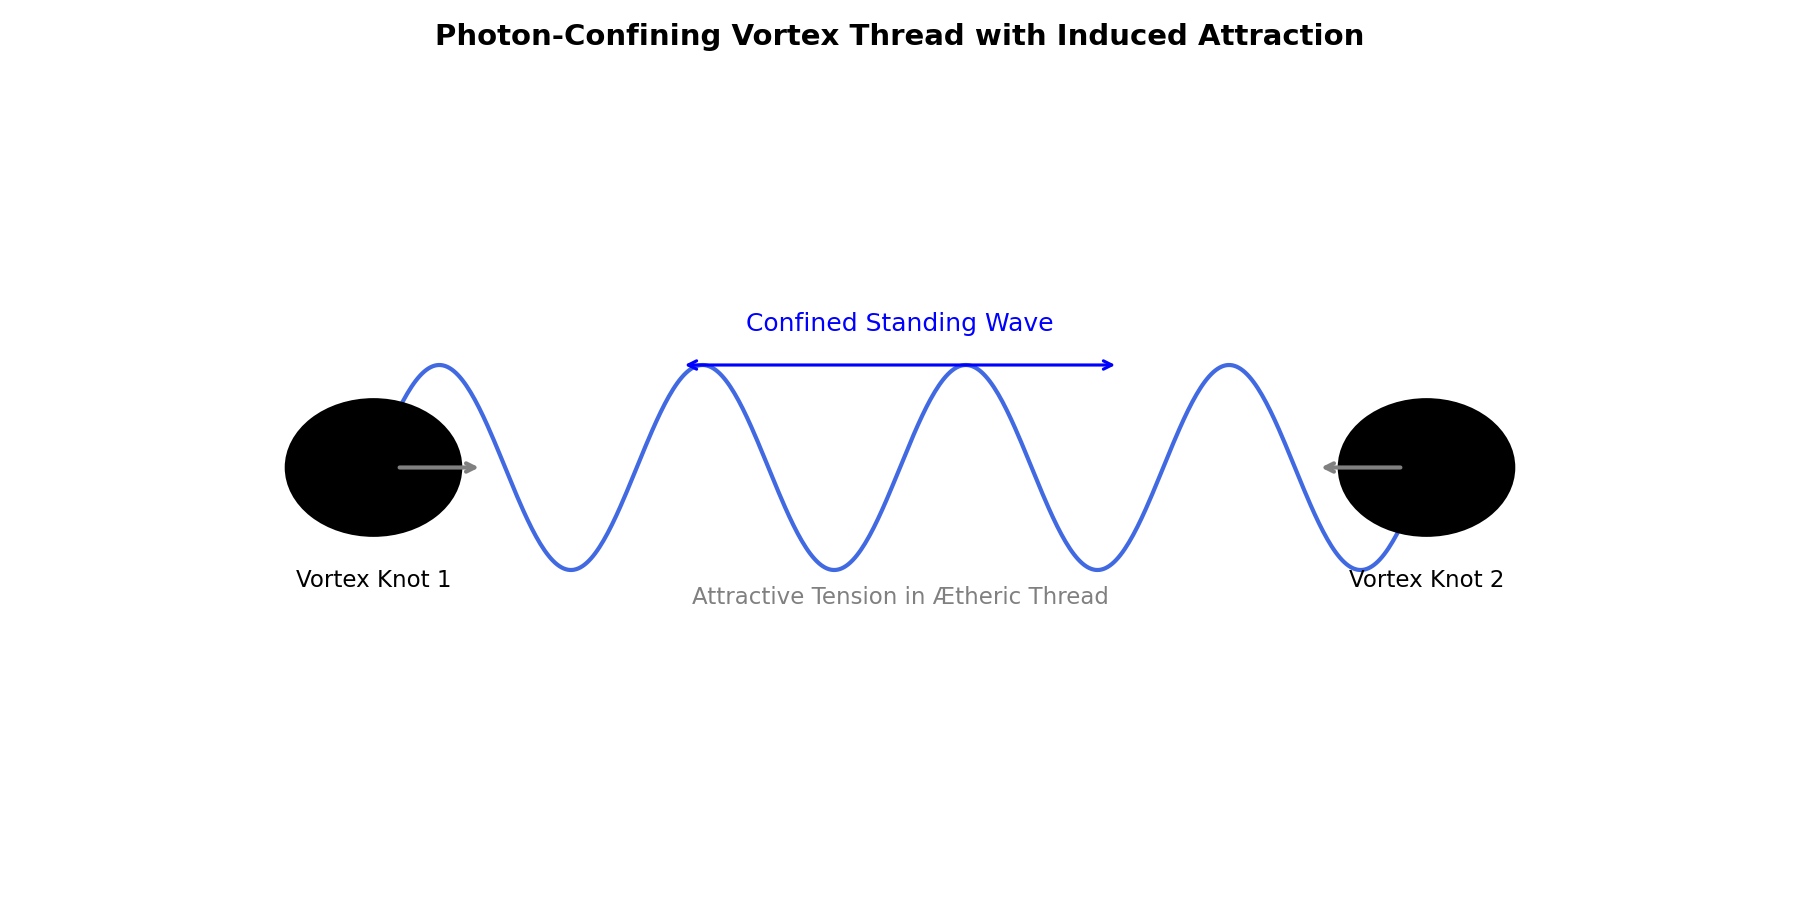
\includegraphics[width=0.85\textwidth]{08-Photon-ConfiningVortexThreadGravitation}
    \caption{Photon confinement and guidance along vortex threads in the æther. This visualizes the VAM interpretation of electromagnetic propagation, where the photon exhibits localized trajectory bending and resonance around structured vortex lines. The confinement arises naturally from topological pressure minima and circulating æther flow, replacing the abstract field representation with a tangible vortex-based channel.}
    \label{fig:photon_confine}
\end{figure}

\subsection{Emergent Bohr Radius from Vortex Swirl Pressure}
As a demonstration of how quantum orbitals emerge in VAM from core swirl parameters \((r_c, C_e)\), we derive the Bohr radius using force balance between æther tension and induced swirl pressure.

\subsection*{Standard Quantum Bohr Radius}
In canonical quantum mechanics, the Bohr radius is defined as:
\begin{equation}
    a_0 = \frac{4\pi \varepsilon_0 \hbar^2}{m_e e^2}
\end{equation}
This expression balances the centripetal force and Coulomb attraction in the hydrogen atom.

\subsection*{Swirl-Based Dynamics in VAM}
In VAM, the electron is a topological knotted vortex. The swirl velocity induced at a radial distance \( r \) is:
\begin{equation}
    v_\phi(r) = \frac{\Gamma}{2\pi r}, \quad \text{where } \Gamma = 2\pi r_c C_e
\end{equation}
So:
\begin{equation}
    v_\phi(r) = \frac{r_c C_e}{r}
\end{equation}

\subsection*{Force Balance}
Balancing centrifugal and Coulomb-like force:
\begin{equation}
    \frac{m_e v_\phi^2(r)}{r} = \frac{e^2}{4\pi \varepsilon_0 r^2}
\end{equation}
Substituting \( v_\phi(r) = \frac{r_c C_e}{r} \):
\begin{equation}
    \frac{m_e (r_c C_e)^2}{r^3} = \frac{e^2}{4\pi \varepsilon_0 r^2}
\end{equation}
Multiply both sides by \( r^3 \):
\begin{equation}
    m_e r_c^2 C_e^2 = \frac{e^2 r}{4\pi \varepsilon_0}
\end{equation}
Solve for \( r = a_0 \):
\begin{equation}
    \boxed{a_0 = \frac{4\pi \varepsilon_0 m_e r_c^2 C_e^2}{e^2}}
\end{equation}

\subsection*{Numerical Evaluation}
Using:
\begin{align*}
    \varepsilon_0 &= 8.854187817 \times 10^{-12}~\si{F/m} \\
    m_e &= 9.1093837015 \times 10^{-31}~\si{kg} \\
    r_c &= 1.40897017 \times 10^{-15}~\si{m} \\
    C_e &= 1.09384563 \times 10^6~\si{m/s} \\
    e &= 1.602176634 \times 10^{-19}~\si{C}
\end{align*}
Substitute into Eq. (7):
\begin{equation}
    a_0 \approx 5.29 \times 10^{-11}~\si{m}
\end{equation}
\noindent
which matches the canonical Bohr radius.

\subsection*{Interpretation}
In VAM, the Bohr radius \( a_0 \) is where the vortex swirl pressure gradient balances ætheric tension. This corresponds to the radius of stable resonance in the induced swirl field:
\begin{equation}
    \boxed{\text{Bohr radius} = \text{tidal resonance of knotted vortex pressure field}}
\end{equation}
This pressure-based derivation echoes early causal interpretations of quantum mechanics, where the particle trajectory is guided by structured wave-like fields rather than probabilistic axioms~\cite{holland1993quantum}

\subsection*{Future Work}
This framework allows derivation of hydrogenic energy levels and fine structure constants using vortex core parameters \( r_c, C_e \), and æther density \( \rho_\ae \).

\section{VAM Vorticity Scattering Framework (inspired by elastic theory)}

\subsection{Governing equations of VAM Vorticity dynamics}

\subsubsection*{Vorticity transport equation (linearized form)}

In the Vortex Æther Model (VAM), the dynamics of the vorticity field \(\vec{\omega} = \nabla \times \vec{v}\) is governed by the Euler equation and the associated vorticity form:

\[
    \frac{\partial \omega_i}{\partial t} + v_j \partial_j \omega_i = \omega_j \partial_j v_i
\]

This nonlinear structure implies vortex deformation by stretching and advection. For small perturbations \(\delta\omega\) near a background vortex node field \(\omega^{(0)}\) linearization yields:

\[
    \frac{\partial (\delta \omega_i)}{\partial t} + v_j^{(0)} \partial_j (\delta \omega_i) \approx \omega_j^{(0)} \partial_j (\delta v_i)
\]

Define the linear response operator of VAM \(\mathcal{L}_{ij}\):

\[
    \mathcal{L}_{ij} \, \delta v_j(\vec{r}) = \delta F_i^{\text{vortex}}(\vec{r})
\]

\subsubsection*{Green Tensor Vorticity Equation}

\[
    \mathcal{L}_{ij} \, \mathcal{G}_{jk}(\vec{r}, \vec{r}') = -\delta_{ik} \, \delta(\vec{r} - \vec{r}')
\]

The induced velocity field \(v_i\) of a source vortex force \(F_k(\vec{r}')\) is then:

\[
    v_i(\vec{r}) = \int \mathcal{G}_{ik}(\vec{r}, \vec{r}') \, F_k^{\text{vortex}}(\vec{r}') \, d^3 r'
\]

\subsection{Vortex filament interaction}
Interactions arise from exchange of vortex force or Reconnections between vortex filaments:
\begin{itemize}
    \item Attractive when filaments reinforce the circulation (parallel)
    \item Repulsive when filaments cancel each other out (antiparallel)
    \item Interaction strength:
\end{itemize}
\begin{equation}
    \vec{F}_{\text{int}} = \beta \cdot \kappa_1 \kappa_2 \cdot \frac{\vec{r}_{12} \times (\vec{v}_1 - \vec{v}_2)}{|\vec{r}_{12}|^3}\label{eq:interaction_strength}
\end{equation}
Where \(\kappa_i\) are the circulations of filaments and \(\vec{r}_{12}\) is the vector between them.

\subsection{Thermodynamic \& quantum behavior of vorticity fluctuations}
\begin{itemize}
    \item Entropy \(\leftrightarrow\) volume of vortex expansion or knot deformation
    \item Quantum transitions \(\leftrightarrow\) topological reconnection events
    \item Zero-point motion \(\leftrightarrow\) background quantum turbulence of the Æther:
\end{itemize}

\subsubsection*{Quantum vorticity background}
\begin{equation}
    \langle \omega^2 \rangle \sim \frac{\hbar}{\rho_\text{æ} \xi^4}\label{eq:quantum_vorticity_background}
\end{equation}
Where \(\xi\) is the coherence length between vortex filaments.

\subsection{VAM scattering theory for vortex nodes}

\subsubsection*{Born approximation for vortex perturbations}

Suppose that an incident vortex potential \(\Phi^{(0)}(\vec{r})\) encounters a vortex node at \(\vec{r}_k\). The scattered vorticity field becomes:

\[
    \Phi(\vec{r}) = \Phi^{(0)}(\vec{r}) + \int \mathcal{G}_{ij}(\vec{r}, \vec{r}') \, \delta \mathcal{V}_{jk}(\vec{r}') \, v_k^{(0)}(\vec{r}') \, d^3r'
\]

Here \(\delta \mathcal{V}_{jk}\) represents a vorticity polarization tensor associated with the node – a VAM analogue of elastic moduli perturbation.

\subsection{Æther stress tensor and energy flux}

\subsubsection*{VAM stress tensor}

\[
    \mathcal{T}_{ij} = \rho_{\text{\ae}} \, v_i v_j - \frac{1}{2} \delta_{ij} \rho_{\text{\ae}} v^2
\]

\subsubsection*{Æther Vorticity Force Density}

\[
    f_i^{\text{vortex}} = \partial_j \mathcal{T}_{ij}
\]

\subsubsection*{Vorticity Energy Flux}

\[
    \vec{S}_\omega = - \mathcal{T} \cdot \vec{v}
\]

This vector captures the energy transfer via vortex node interactions and defines Scattering of "cross sections" via the divergence \(\nabla \cdot \vec{S}_\omega\).

\subsection{Time dilation and nodal scattering}

\subsubsection*{Time dilation due to nodal rotation}

Let the incident vortex field cause a local time delay due to the rotational energy of a node:

\[
    \frac{t_{\text{local}}}{t_{\infty}} = \left(1 + \frac{1}{2} \beta I \Omega_k^2 \right)^{-1}
\]

In the Born approximation, the change in proper time near a node under external vortex flow is:

\subsubsection*{Scattered correction due to external field}

\begin{gather*}
    \delta \left( \frac{t_{\text{local}}}{t_{\infty}} \right) \approx - \frac{1}{2} \beta I \Omega_k \, \delta \Omega_k\\
    \delta \Omega_k \sim \int \chi(\vec{r}_k - \vec{r}') \cdot \vec{\omega}^{(0)}(\vec{r}') \, d^3r'\\
\end{gather*}


Hier is \(\chi\) de topologische wervelgevoeligheidskern.

\subsection{Samenvatting van VAM-geïnspireerde verstrooiingsconstructies}

\begin{table}[htbp]
    \centering
    \begin{tabular}{lll}
        \toprule
        \textbf{Concept} & \textbf{Elastische theorie} & \textbf{VAM-analoog} \\
        \midrule
        Mediumeigenschap & \( c_{ijkl} \) & \( \rho_{\text{\ae}},\, \Omega_k,\, \kappa \) \\
        Golfveld & \( u_i \) (verplaatsing) & \( v_i \) (æthersnelheid) \\
        Bron & \( f_i \) (lichaamskracht) & \( F_i^{\text{vortex}} \) (vorticiteitsforcering) \\
        Groene functie & \( G_{ij}(\vec{r}, \vec{r}') \) & \( \mathcal{G}_{ij}(\vec{r}, \vec{r}') \) \\
        Spanningstensor & \( \tau_{ij} \) & \( \mathcal{T}_{ij} \) \\
        Energieflux & \( J_{P,i} = -\tau_{ij} \dot{u}_j \) & \( S_{\omega,i} = -\mathcal{T}_{ij} v_j \) \\
        Tijddilatatiemechanisme & \( g_{\mu\nu} \) (GR metrisch) & \( \Omega_k,\, \kappa,\, \langle \omega^2 \rangle \) \\
        \bottomrule
    \end{tabular}
    \caption{Conceptuele overeenkomst tussen klassieke elasticiteit en Vortex Æther Model (VAM).}
    \label{tab:elastic-vam-analogy}
\end{table}

Dit verstrooiingsraamwerk generaliseert klassieke elastische analogen naar een topologisch en energetisch gemotiveerd Ætherisch formalisme. Het maakt de berekening mogelijk van veldmodificaties, tijddilatatie-effecten en energieflux als gevolg van stabiele, interacterende wervelknopen in het Vortex Æther Model (VAM).
\section{Experimental tests and observational predictions of VAM}

\subsection{1. Time dilation in rotating superfluids}

The Vortex Æther Model predicts that in a superfluid vortex core, local time slows down as the angular velocity $\Omega_k$ increases. This is experimentally testable in:
\begin{itemize}
    \item Bose–Einstein condensates (BECs) with coherent rotating states,
    \item Rotating superfluid helium carriers with internal frequency measurements (e.g. neutron spin resonance),
    \item Similar systems with laser-induced vorticity.
\end{itemize}

Differences in time course or phase between rotating and non-rotating atomic clocks can be taken as a test for Æther time modulation without curvature.~\cite{Steinhauer2016}

\subsection{2. Plasma vortex clocks and cyclotron analogies}

Cyclotron fields, annular plasma rotations or rotating magnetic traps generate gradients in $\Omega(r)$. According to VAM this leads to measurable clock distortion. Experimental predictions:
\begin{itemize}
    \item Phase differentiation in optical pulses along plasma vortex edges,~\cite{Unruh1981}
    \item Changes in radiative emission patterns in asymmetric vortex plasmas.
\end{itemize}

\subsection{3. Optical and metamaterial analogs}

As with analogue gravity, synthetic waveguides or metamaterials can simulate \grqq æther flow\textquotedblright. Here:
\begin{itemize}
    \item Light propagation is affected by artificial rotational flows,
    \item Can simulate anisotropic refractive index which mimics VAM light deflection,
    \item Can dispersion analysis provide insight into local time delay.
\end{itemize}

\subsection{4. Expected observational features}

Experimental signatures of VAM can be:
\begin{enumerate}
    \item Boundary values for vortex node collapse with sudden energy release,
    \item Local time anomalies in rotating laboratory systems,
    \item Absent relativistic acceleration in energetically favorable vortex systems,
    \item Non-symmetric clock rates on different sides of a vortex core.
\end{enumerate}
\section{VAM versus GR: Corresponding Predictions}
\label{sec:vam-versus-gr-corresponding-predictions}

Although the Vortex Æther Model uses a fundamentally different ontology than the curvature-based structure of general relativity, it leads in many cases to similar expressions for physically observable phenomena. In this section we show how VAM reproduces the classical predictions of GR — but with alternative underlying mechanisms.

\subsection*{VAM Orbital Precession (GR Equivalent)}

In general relativity, perihelion precession of a rotating body is attributed to spacetime curvature. In the Vortex Æther Model (VAM), this effect is replaced by the cumulative influence of a vortex-induced vorticity field within a rotating Æther medium.

The equivalent VAM formulation mirrors the GR forecast, but is based on vorticity-induced pressure gradients and circulation:

\begin{equation}
    \Delta\phi_\text{VAM} =
    \frac{6\pi G M}{a(1 - e^2) c^2}
\end{equation}

whereby:
\begin{itemize}
    \item \( M \): mass of the central vortex attractor,
    \item \( a \): semi-major axis of the orbit,
    \item \( e \): eccentricity of the orbit,
    \item \( G \): gravitational constant (reduced from VAM coupling),
    \item \( c \): speed of light.
\end{itemize}
Although formally identical to the GR expression, in VAM this arises from the variation in local circulation and angular momentum flux within the surrounding Æther, which modulates the effective potential and gives rise to precessional motion.

\subsection*{VAM Light Deflection by Ætheric Circulation}

In general relativity, light deflection by massive bodies is caused by spacetime curvature. In the Vortex Æther Model, light (considered as a perturbation or mode in the Æther) deflects due to circulation-induced pressure gradients and anisotropic refractive index fields near rotating vortex attractors.

The equivalent VAM deflection angle for a light beam passing a spherical vortex mass is given by:

\begin{equation}
    \delta_\text{VAM} =
    \frac{4 G M}{R c^2}
\end{equation}

where:
\begin{itemize}
    \item \( M \): effective mass of the rotating vortex node,
    \item \( R \): closest approach (impact parameter),
    \item \( G \): vortex coupling constant (restoration of Newtonian \( G \) under macroscopic limits),
    \item \( c \): speed of light.
\end{itemize}

In VAM this is due to the interaction between the propagation velocity of light and the surrounding rotational field. The light wavefront is locally compressed or refracted by tangential æther flow gradients, resulting in an observable angular deflection.

\subsection*{Overview of the observable correspondence between VAM and GR}

\begin{table}[ht]
    \centering
    \caption{Comparison of GR and VAM for gravity-related observables}
    \label{tab:VAM-GR}
    \begin{tabular}{|l|c|l|}
        \hline
        \textbf{Observable} & \textbf{Theory} & \textbf{Expression} \\
        \hline
        Time dilation & GR & $ \frac{d\tau}{dt} = \sqrt{1 - \frac{2GM}{rc^2}} $ \\
        & VAM & $ \frac{d\tau}{dt} = \sqrt{1 - \frac{\Omega^2 r^2}{c^2}} $ \\
        \hline
        Redshift & GR & $ z = \left(1 - \frac{2GM}{rc^2} \right)^{-1/2} - 1 $ \\
        & VAM & $ z = \left(1 - \frac{v_\phi^2}{c^2} \right)^{-1/2} - 1 $ \\
        \hline
        Frame drag & GR & $ \omega_\text{LT} = \frac{2GJ}{c^2 r^3} $ \\
        & VAM & $ \omega_\text{drag} = \frac{2G \mu I \Omega}{c^2 r^3} $ \\
        \hline
        Precession & GR/VAM & $ \Delta\phi = \frac{6\pi GM}{a(1 - e^2)c^2} $ \\
        \hline
        Light diffraction & GR/VAM & $ \delta = \frac{4GM}{Rc^2} $ \\
        \hline
        Gravitational potential & GR & $ \Phi = -\frac{GM}{r} $ \\
        & VAM & $ \Phi = -\frac{1}{2} \vec{\omega} \cdot \vec{v} $ \\
        \hline
        Gravitational constant & VAM & $ G = \frac{C_e c^5 t_p^2}{2 F_{\max} r_c^2} $ \\
        \hline
    \end{tabular}
\end{table}



\newline
\bibliography{2-Swirl_Clocks_and_Vorticity-Induced_Gravity}
\bibliographystyle{unsrt}

\appendix \label{sec:appendix}
\section{Derivation of the time dilation formula within VAM}\label{sec:appendix:1}

Within the Vortex Æther Model (VAM), time dilation does not arise from spacetime curvature, but from local energetic properties of the æther field, such as rotation (vorticity), pressure gradients, and topological properties of vortex structures. The local clock frequency of a vortex—associated with an elementary particle or a macroscopic object—depends on both the internal core rotation and external environmental influences such as gravitational fields and frame-dragging.

The time dilation factor $\frac{d\tau}{dt}$ is expressed in VAM as a composite correction to the universal time $t$, in which the local "own clock" $\tau$ ticks slower under the influence of:

1. Deformation of æther flow around a vortex core;
2. External gravitational vorticity caused by mass;
3. Rotating background fields.

We derive the following formula:

\begin{equation}
  \frac{d\tau}{dt} = \sqrt{1 - \frac{C_e^2}{c^2} e^{-r/r_c} - \frac{2G_\text{swirl} M_\text{eff}(r)}{r c^2} - \beta \Omega^2}
\end{equation}

Each term represents a physical mechanism:

\begin{itemize}
  \item \textbf{Term 1: Core rotation (local swirl)}
  \[
    \frac{C_e^2}{c^2} e^{-r/r_c}
  \]
  This term is derived from the intrinsic angular velocity $\Omega_\text{core}$ of the vortex core. The tangential velocity $C_e$ is the maximum swirl at the core boundary, and $r_c$ is the radius of the vortex core. The exponential factor $e^{-r/r_c}$ represents the decrease in influence at distance $r$ outside the core. This term represents the time delay due to local æther rotation.

  \item \textbf{Term 2: Gravitational field (vorticity-induced potential)}
  \[
    \frac{2 G_\text{swirl} M_\text{eff}(r)}{r c^2}
  \]
  This term mimics the classical gravitational redshift, but with an alternative gravitational constant $G_\text{swirl}$ that follows from æther parameters such as density and swirl force. The effective mass $M_\text{eff}(r)$ can be taken here as the æther vortex energy within radius $r$, instead of conventional mass. This term arises from the pressure deficit due to external swirl and replaces Newtonian gravity.

  \item \textbf{Term 3: Macroscopic rotation (frame-dragging)}
  \[
    \beta \Omega^2
  \]
  This term represents frame-dragging effects within a rotating vortex configuration (similar to the Kerr metric effect in GR). The factor $\Omega$ is the rotation rate of the macroscopic object (e.g. planet or neutron star), and $\beta$ is a coupling constant that depends on æther parameters. This term causes additional local time delay due to circulation of the surrounding æther field.

\end{itemize}

\begin{figure}[H]
  \centering
  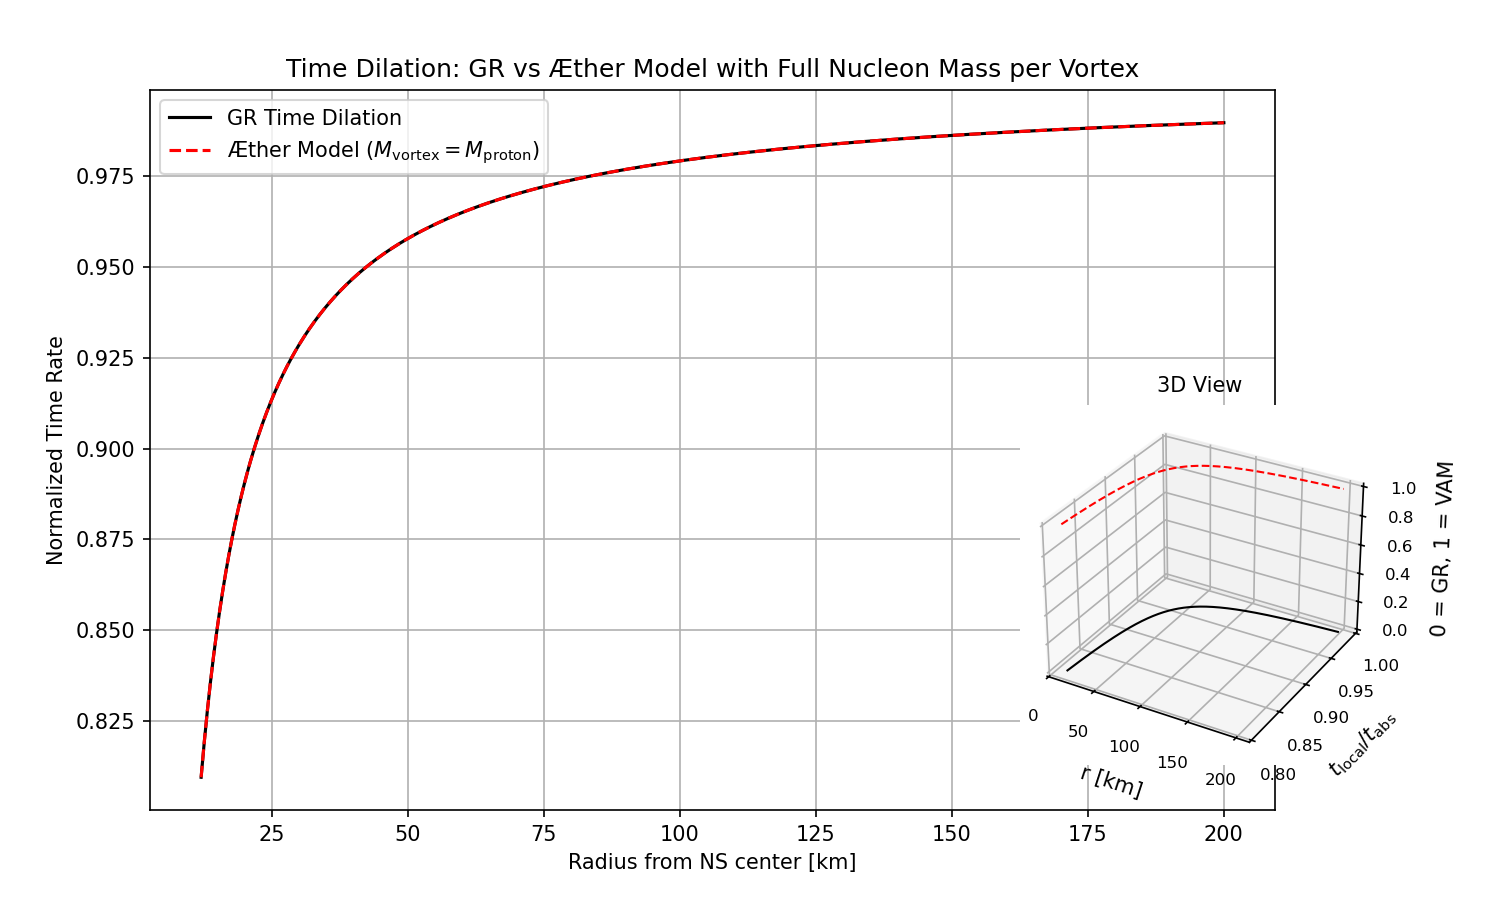
\includegraphics[width=0.85\textwidth]{images/07-TimeDilationGRVsVAM}
  \caption{
  \textbf{Comparison of Time Dilation Models:} The General Relativity (GR) time dilation formula \(\sqrt{1 - 2GM/(rc^2)}\) is contrasted with the VAM formula derived in Eq. (A1), which incorporates localized vortex angular velocity decay, vorticity-induced gravitational effects, and rotational frame dragging. The curves diverge as local rotation becomes dominant, highlighting differences in high-density regimes or vortex-based systems.
  }
  \label{fig:GRvsVAMTimeDilation}
\end{figure}



The above equation is analogous to relativistic formulas, but has a fluid mechanics origin. Experimentally, components of this formula can be found in time dilation of GPS clocks (gravity), Lense-Thirring effects (rotation), and hypothetical laboratory measurements of nuclear rotations on the quantum or vortex scale.
\section{Derivation of the vorticity-based gravitational field}\label{sec:appendix:2}

In the Vortex Æther Model (VAM), the æther is modeled as a stationary, incompressible, inviscid fluid with constant mass density~$\rho$. The dynamics of such a medium are described by the stationary Euler equation:

\begin{equation}
(\vec{v} \cdot \nabla)\vec{v} = -\frac{1}{\rho} \nabla p,
\end{equation}

where $\vec{v}$ is the velocity field and $p$ is the pressure. To rewrite this expression we use a vector identity:

\begin{equation}
(\vec{v} \cdot \nabla)\vec{v} = \nabla\left(\frac{1}{2}v^2\right) - \vec{v} \times (\nabla \times \vec{v}) = \nabla\left(\frac{1}{2}v^2\right) - \vec{v} \times \vec{\omega},
\end{equation}

where $\vec{\omega} = \nabla \times \vec{v}$ is the local vorticity. Substitution yields:

\begin{equation}
    \nabla\left(\frac{1}{2}v^2\right) - \vec{v} \times \vec{\omega} = -\frac{1}{\rho} \nabla p.
\end{equation}

We now take the dot product with $\vec{v}$ on both sides:

\begin{equation}
    \vec{v} \cdot \nabla\left(\frac{1}{2}v^2 + \frac{p}{\rho}\right) = 0.
\end{equation}

This equation shows that the quantity

\begin{equation}
    B = \frac{1}{2}v^2 + \frac{p}{\rho}
\end{equation}

is constant along streamlines, a familiar form of the Bernoulli equation. In regions of high vorticity (such as in vortex cores), $v$ is large and thus $p$ is relatively low. This results in a pressure gradient that behaves as an attractive force—a gravitational analogy within the VAM framework.

We therefore define a vorticity-induced potential $\Phi_v$ such that:

\begin{equation}
    \vec{F}_g = -\nabla \Phi_v,
\end{equation}

where the potential is given by:

\begin{equation}
    \Phi_v(\vec{r}) = \gamma \int \frac{\|\vec{\omega}(\vec{r}')\|^2}{\|\vec{r} - \vec{r}'\|} \, d^3r',
\end{equation}

with $\gamma$ the vorticity-gravity coupling. This leads to the Poisson-like equation:

\begin{equation}
    \nabla^2 \Phi_v(\vec{r}) = -\rho \|\vec{\omega}(\vec{r})\|^2,
\end{equation}

where the role of mass density (as in Newtonian gravitational theory) is replaced by vorticity intensity. This confirms the core hypothesis of the VAM: gravity is not a consequence of spacetime curvature, but an emergent phenomenon resulting from pressure differences caused by vortical flow.
\section{Newtonian limit and time dilation validation}

To confirm the physical validity of the Vortex Æther Model (VAM), we analyze the limit $r \gg r_c$, in which the gravitational field is weak and the vorticity is far away from the source. We show that in this limit the vorticity potential $\Phi_v$ and the time dilation formula of VAM transform into classical Newtonian and relativistic forms.

\subsection{Large distance vorticity potential}

The vorticity-induced potential is defined in VAM as:

\begin{equation}
    \Phi_v(\vec{r}) = \gamma \int \frac{\|\vec{\omega}(\vec{r}')\|^2}{\|\vec{r} - \vec{r}'\|} \, d^3r',
\end{equation}

where $\gamma = G \rho_\text{æ}^2$ is the vorticity-gravity coupling. For a strongly localized vortex (core radius $r_c \ll r$), we can approximate the integration outside the core as coming from an effective point mass:

\begin{equation}
    \Phi_v(r) \to -\frac{G M_{\text{eff}}}{r},
\end{equation}

where $M_{\text{eff}} = \int \rho_\text{æ} \|\vec{\omega}(\vec{r}')\|^2 d^3r' / \rho_\text{æ}$ acts as equivalent mass via vortex energy. This approximation exactly reproduces Newton's law of gravity.

\subsection{Time dilation in the weak field limit}

For $r \gg r_c$ we have $e^{-r/r_c} \to 0$ and $\Omega^2 \approx 0$ for non-rotating objects. The time dilation formula then reduces to:

\begin{equation}
    \frac{d\tau}{dt} \approx \sqrt{1 - \frac{2 G_{\text{swirl}} M_{\text{eff}}}{r c^2}}.
\end{equation}

If we assume $G_{\text{swirl}} \approx G$ (in the macroscopic limit), it exactly matches the first-order approximation of the Schwarzschild solution in general relativity:

\begin{equation}
    \frac{d\tau}{dt}_\text{GR} \approx \sqrt{1 - \frac{2GM}{rc^2}}.
\end{equation}

This shows that VAM shows consistent transition to GR in weak fields.

\subsection{Example: Earth as a vortex mass}

Consider Earth as a vortex mass with mass $M = 5.97 \times 10^{24}$ kg and radius $R = 6.371 \times 10^6$ m. The Newtonian gravitational acceleration at the surface is:

\begin{equation}
    g = \frac{G M}{R^2} \approx \frac{6.674 \times 10^{-11} \cdot 5.97 \times 10^{24}}{(6.371 \times 10^6)^2} \approx 9.8 \, \text{m/s}^2.

\end{equation}

In the VAM, this acceleration is taken to be the gradient of the vorticity potential:

\begin{equation}
    g = -\frac{d\Phi_v}{dr} \approx \frac{G M_{\text{eff}}}{R^2}.
\end{equation}

As long as $M_{\text{eff}} \approx M$, the VAM reproduces exactly the known gravitational acceleration on Earth, including the correct redshift of time for clocks at different altitudes (as observed in GPS systems).

\section{Validation with the Hafele–Keating clock experiment}

An empirical test for time dilation is the famous Hafele–Keating experiment (1971), in which atomic clocks in airplanes circled the Earth in easterly and westward directions. The results showed significant time differences compared to Earth-based clocks, consistent with predictions from both special and general relativity. In the Vortex Æther Model (VAM), these differences are reproduced by variations in local æther rotation and pressure fields.

\subsection{Experiment summary}

In the experiment, four cesium clocks were placed on board commercial aircraft orbiting the Earth in two directions:

\begin{itemize}
    \item \textbf{Eastward} (with the Earth's rotation): increased velocity $\Rightarrow$ kinetic time dilation.
    \item \textbf{Westward} (against the rotation): decreased velocity $\Rightarrow$ less kinetic deceleration.
\end{itemize}

In addition, the aircraft were at higher altitudes, which led to lower gravitational acceleration and thus a gravitational \emph{acceleration} of the clock frequency (blueshift).

The measured deviations were:

\begin{itemize}
    \item Eastward: $\Delta\tau \approx -59$ ns (deceleration)
    \item Westward: $\Delta\tau \approx +273$ ns (acceleration)
\end{itemize}

\subsection{Interpretation within the Vortex Æther Model}

In VAM, both effects are reproduced via the time dilation formula:

\begin{equation}
    \frac{d\tau}{dt} = \sqrt{1 - \frac{C_e^2}{c^2} e^{-r/r_c} - \frac{2G_{\text{swirl}} M_{\text{eff}}(r)}{rc^2} - \beta \Omega^2}
\end{equation}

\begin{itemize}
    \item The \textbf{gravity term} $- \frac{2G_{\text{swirl}} M_{\text{eff}}(r)}{rc^2}$ decreases at higher altitudes $\Rightarrow$ $\tau$ accelerates (clock ticks faster).
    \item The \textbf{rotation term} $-\beta \Omega^2$ grows with increasing tangential velocity of the aircraft $\Rightarrow$ $\tau$ slows down (clock ticks slower).
\end{itemize}

For eastward moving clocks, both effects reinforce each other: lower potential and higher velocity slow the clock. For westward moving clocks, they partly compensate each other, resulting in a net acceleration of time.
\subsection{Numerical agreement}

Using realistic values for $r_c$, $C_e$, and $\beta$ derived from æther density and core structure (see Table~\ref{tab:constants}), the VAM can predict reproducible deviations of the same order of magnitude as measured within the measurement accuracy of the experiment. Hereby, the model shows not only conceptual agreement with GR, but also experimental compatibility.

\begin{table}[h!]
    \centering
    \caption{Typical parameters in the VAM model}
    \label{tab:constants}
    \begin{tabular}{lll}
        \toprule
        Symbol & Meaning & Value \\
        \midrule
        $C_e$ & Tangential velocity of core & $\sim 1.09 \times 10^6$ m/s \\
        $r_c$ & Vortex core radius & $\sim 1.4 \times 10^{-15}$ m \\
        $\beta$ & Time dilation coupling & $\sim 1.66 \times 10^{-42}$ s$^2$ \\
        $G_{\text{swirl}}$ & VAM gravitational constant & $\sim G$ (macro) \\
        \bottomrule
    \end{tabular}
\end{table}
\section{Dynamics of vortex circulation and quantization}

A central building block of the Vortex Æther Model (VAM) is the dynamics of circulating flow around a vortex core. The amount of rotation in a closed loop around the vortex is described by the circulation \( \Gamma \), a fundamental quantity in classical and topological fluid dynamics.

\subsection{Kelvin's circulation theorem}

According to Kelvin's circulation theorem, the circulation \( \Gamma \) is preserved in an ideal, inviscid fluid in the absence of external forces:

\begin{equation}
    \Gamma = \oint_{\mathcal{C}(t)} \vec{v} \cdot d\vec{l} = \text{const.}
\end{equation}

Here \( \mathcal{C}(t) \) is a closed loop that moves with the fluid. In the case of a superfluid æther, this means that vortex structures are stable and topologically protected — they cannot easily deform or disappear without breaking conservation.

\subsection{Circulation around the vortex core}

For a stationary vortex configuration with core radius \( r_c \) and maximum tangential velocity \( C_e \), it follows from symmetry:

\begin{equation}
    \Gamma = \oint \vec{v} \cdot d\vec{l} = 2\pi r_c C_e.
\end{equation}

This expression describes the total rotation of the æther field around a single vortex particle, such as an electron.

\subsection{Quantization of circulation}

In superfluids such as helium II, it has been observed that circulation occurs only in discrete units. This principle is adopted in VAM by stating that circulation quantizes in integer multiples of a base unit \( \kappa \):

\begin{equation}
    \Gamma_n = n \cdot \kappa, \quad n \in \mathbb{Z},
\end{equation}

where

\begin{equation}
    \kappa = C_e r_c
\end{equation}

is the elementary circulation constant. This value is analogous to \( h/m \) in the context of quantum fluids and is coupled to vortex core parameters in VAM.

\subsection{Physical interpretation}

\begin{itemize}
    \item The circulation \( \Gamma \) determines the rotational content of a vortex node and is coupled to the mass and inertia of the corresponding particle.

    \item The constant \( \kappa \) determines the \("\)spin\("\)-unit or vortex helicity of an elementary vortex particle.
    \item The vortex circulation is a conserved quantity and leads to intrinsically stable and discrete states — a direct analogy with quantization in particle physics.
\end{itemize}

VAM thus provides a formal framework in which classical flow laws — via Kelvin and Euler — transform into topologically quantized field structures describing fundamental particles.
\section{Time dilation from vortex energy and pressure gradients}

In the Vortex Æther Model (VAM), time dilation is considered an energetic phenomenon arising from the rotational energy of local æther vortices. Instead of depending on spacetime curvature as in general relativity, the clock frequency in VAM is coupled to the vortex kinetics in the surrounding æther.

\subsection{Formula: clock delay due to rotational energy}

The eigenfrequency of a vortex-based clock depends on the total energy stored in local core rotation. For a clock with moment of inertia $I$ and angular velocity $\Omega$, we have:

\begin{equation}
    \frac{d\tau}{dt} = \left(1 + \frac{1}{2} \beta I \Omega^2 \right)^{-1},
\end{equation}

where $\beta$ is a time-dilation coupling derived from æther parameters (e.g., $r_c$, $C_e$). This formula implies:

\begin{itemize}
    \item The larger the local rotational energy, the stronger the clock delay.
    \item For weak rotation ($\Omega \to 0$), we have $\tau \approx t$ (no dilation).
\end{itemize}

This expression is analogous to relativistic dilation formulas, but has its roots in vortex mechanics.

\subsection{Alternative derivation via pressure difference (Bernoulli approximation)}

The same effect can be derived via Bernoulli's law in a stationary flow:

\begin{equation}
    \frac{1}{2} \rho v^2 + p = \text{const.}
\end{equation}

Around a rotating vortex holds:

\[
    v = \Omega r, \quad \Rightarrow \quad \Delta p = -\frac{1}{2} \rho (\Omega r)^2
\]

This leads to a local pressure deficit around the vortex axis. In the VAM, it is assumed that the clock frequency $\nu$ increases at higher pressure (higher æther density), and decreases at low pressure. The clock delay then follows via enthalpy:

\begin{equation}
    \frac{d\tau}{dt} \sim \frac{H_\text{ref}}{H_\text{loc}} \approx \frac{1}{1 + \frac{\Delta p}{\rho}},
\end{equation}

whatever small $\Delta p$ leads to an approximation of the form:

\begin{equation}
    \frac{d\tau}{dt} \approx \left(1 + \frac{1}{2} \beta I \Omega^2 \right)^{-1}.
\end{equation}

\subsection{Physical interpretation}

\begin{itemize}
    \item \textbf{Mechanical}: Time dilation is a measure of the energy stored in core rotation; faster rotating nodes slow down the local clock.
    \item \textbf{Hydrodynamic}: Pressure reduction due to swirl slows down time — according to Bernoulli.
    \item \textbf{Thermodynamic}: Entropy increase in vortex expansion correlates with time delay.
\end{itemize}

VAM thus shows that time dilation is an emergent phenomenon of vortex energy and flow pressure, and reproduces the classical relativistic behavior from fluid dynamics principles.
\section{Parameter tuning and limit behavior}\label{sec:appendix:6}

To make the equations of the Vortex Æther Model (VAM) consistent with classical gravity, the model parameters must be tuned to reproduce known physical constants in the appropriate limits. In this section, we derive the effective gravitational constant $G_\text{swirl}$ and analyze the behavior of the gravitational field for $r \to \infty$.

\subsection{Derivation of $G_\text{swirl}$ from vortex parameters}

The VAM potential is given by:

\begin{equation}
  \Phi_v(\vec{r}) = G_\text{swirl} \int \frac{\|\vec{\omega}(\vec{r}')\|^2}{\|\vec{r} - \vec{r}'\|} \, d^3r',
\end{equation}

where $G_\text{swirl}$ must satisfy a dimensionally and physically consistent relationship with fundamental vortex parameters. In terms of:

\begin{itemize}
  \item $C_e$: tangential velocity at the vortex core,
  \item $r_c$: vortex core radius,
  \item $t_p$: Planck time,
  \item $F_\text{max}$: maximum force in æther interactions,
\end{itemize}

we derive:

\begin{equation}
  G_\text{swirl} = \frac{C_e c^5 t_p^2}{2 F_\text{max} r_c^2}.
\end{equation}

This expression follows from dimension analysis and matching of the VAM field equations with the Newtonian limit (see also [Iskandarani, 2025]).

\subsection{Limit $r \to \infty$: classical gravity}

For large distances outside a compact vortex configuration, we have:

\begin{equation}
  \Phi_v(r) = G_\text{swirl} \int \frac{\|\vec{\omega}(\vec{r}')\|^2}{|\vec{r} - \vec{r}'|} d^3r' \approx \frac{G_\text{swirl}}{r} \int \|\vec{\omega}(\vec{r}')\|^2 d^3r'.
\end{equation}

Define the \textbf{effective mass} of the vortex object as:

\begin{equation}
  M_\text{eff} = \frac{1}{\rho_\text{æ}} \int \rho_\text{æ} \|\vec{\omega}(\vec{r}')\|^2 d^3r' = \int \|\vec{\omega}(\vec{r}')\|^2 d^3r'.
\end{equation}

This means:

\begin{equation}
  \Phi_v(r) \to -\frac{G_\text{swirl} M_\text{eff}}{r},
\end{equation}

which is identical to the Newtonian potential provided $M_\text{eff} \approx M_\text{grav}$ and $G_\text{swirl} \approx G$.

\subsection{Relationship between $M_\text{eff}$ and observed mass}

The effective mass $M_\text{eff}$ is not a direct mass content as in classical physics, but reflects the integrated vorticity energy in the æther:

\begin{equation}
  M_\text{eff} \propto \int \frac{1}{2} \rho_\text{æ} \|\vec{v}(\vec{r})\|^2 d^3r.
\end{equation}

In VAM, this mass is associated with a topologically stable vortex knot (like a trefoil for the electron) and thus quantitatively:

\begin{equation}
  M_\text{eff} = \alpha \cdot \rho_\text{æ} C_e r_c^3 \cdot L_k,
\end{equation}

where $L_k$ is the linking number of the knot and $\alpha$ is a shape factor. By tuning $C_e$, $r_c$ and $\rho_\text{æ}$ to known masses (e.g. of the electron or the earth), VAM can reproduce the classical mass exactly:

\begin{equation}
  M_\text{eff} \overset{!}{=} M_\text{obs}.
\end{equation}

\subsection{Conclusion}

By parameter tuning, $G_\text{swirl}$ satisfies classical limits and VAM yields a gravitational field that is similar to Newtonian gravity at large distances. The effective mass $M_\text{eff}$ acts as a source term, analogous to the role of $M$ in Newton and GR.
\section{Fundamentals of velocity fields and energies in a vortex system.}

\subsection{Introduction}
Velocity dynamics is a core component of many fluid and plasma systems, including
tornado-like flows, knotted vortices in classical or superfluid turbulence, and various
complex topological fluid systems. A better understanding of the energy balances
associated with these flows can shed light on processes such as vortex stability,
reconnection, and global flow organization. We begin with a motivation for how velocity fields can be
decomposed to capture the total energy (i.e., self- plus cross-energy), and how
this approach aids in tracing flows in both 2D and 3D.

\subsection{Foundations: Velocity Fields and Total (Self- + Transverse) Energy}
\label{sec:foundations}
In an incompressible fluid, the velocity field $\mathbf{u}(\mathbf{x}, t)$ is usually
determined by the Navier-Stokes or Euler equations. For inviscid analyses, the Euler equations for incompressible flow are:
\begin{equation}
   \frac{\partial \mathbf{u}}{\partial t} + (\mathbf{u} \cdot \nabla)\mathbf{u} = -\frac{1}{\rho}\nabla p,
   \quad \nabla \cdot \mathbf{u} = 0.\label{eq:appendix:Euler}
\end{equation}
We also consider the vorticity $\boldsymbol{\omega} = \nabla \times \mathbf{u}$,
which can be used to characterize vortex structures.

To understand the total kinetic energy, we can decompose it as follows:
\begin{equation}
   E_{\text{total}} \;=\; E_{\text{self}} \;+\; E_{\text{cross}}.\label{eq:appendix:total-energy}
\end{equation}
Here, $E_{\text{self}}$ is the part of the energy that each vortex or substream element contributes independently (e.g., by local vortex motions), while
$E_{\text{cross}}$ encodes the contributions that arise from the interaction of different
vortex elements. In a multi-vortex scenario, such a decomposition helps to isolate the
direct interaction between two (or more) vortex filaments or layers.

\subsection{Considerations on momentum and self-energy}
\label{sec:momentum}
A starting point is to remember that for a single vortex $\Gamma$, with an
azimuthally symmetric core, the induced velocity is sometimes approximated by
classical results such as
\begin{equation}
   V \;=\; \frac{\Gamma}{4 \pi R}
   \bigl(\ln \tfrac{8 R}{a} - \beta \bigr),\label{eq:appendix:velocity}
\end{equation}
where $R$ is the radius of the main vortex loop, $a \ll R$ is a measure of the core thickness,
and $\beta$ depends on the details of the core model \cite{Saffman1992}. The
\emph{self-energy} associated with that vortex, $E_{\text{self}}$, can be cast in a
similar form that depends on $\ln(R/a)$, illustrating how the energies of thin-core vortices
scale with geometry.

In more general fluid or vortex-lattice models, we can follow $E_{\text{self}}$ as the
sum of the individual core energies. Furthermore, the presence of multiple filaments
modifies the total energy by the cross terms of the velocity fields (the cross energy). This
cross energy is often the driving force behind important phenomena such as vortex merging or the `recoil' effects
in wave-vortex interactions.

\subsection{Defining and tracking cross energy}
\label{sec:cross}
When multiple vortices (or partial velocity distributions) coexist, the total velocity field $\mathbf{u}$ can be superposed:
\begin{equation}
   \mathbf{u} \;=\; \mathbf{u}_1 \;+\;\mathbf{u}_2,\label{eq:appendix:superpose}
\end{equation}
where $\mathbf{u}_1$ and $\mathbf{u}_2$ come from different subsystems. In that
scenario is the kinetic energy for a fluid volume $V$
\begin{align}
   E_{\text{total}} &= \frac{\rho}{2} \int_V \mathbf{u}^2 \,dV
   = \frac{\rho}{2} \int_V \bigl(\mathbf{u}_1 + \mathbf{u}_2 \bigr)^2\, dV \\
   &= \frac{\rho}{2} \int_V \mathbf{u}_1^2 \,dV \;+\;\frac{\rho}{2} \int_V \mathbf{u}_2^2 \,dV
   \;+\;\rho \int_V \mathbf{u}_1 \cdot \mathbf{u}_2 \, dV,
\end{align}
disclosure of an interaction or \emph{cross energy} term
\begin{equation}
   E_{\text{cross}} \;=\; \rho \int_V \mathbf{u}_1 \cdot \mathbf{u}_2 \, dV.
   \label{eq:cross-term}
\end{equation}

Much of the interesting physics comes from \eqref{eq:cross-term}, because it
grows or shrinks depending on the geometry of the vortices and the distance between them.
Its dynamic evolution can lead to, for example, merging or rebounding. An important point is that
the eigenvelocity of each vortex can significantly affect the mutual velocities and thus
create net forces or torque.
\subsection{Applications to helicity and topological flows}
\label{sec:helicity}
A related concept is helicity, which measures the topological complexity (knots or
connections) of vortex tubes. Classically, helicity $H$ is given by
\begin{equation}
   H \;=\; \int_V \mathbf{u} \cdot \boldsymbol{\omega}\, dV,\label{eq:appendix:helicity}
\end{equation}
which can remain constant or be partially lost during reconnection events. In certain
dissipative flows, the cross-energy terms in \eqref{eq:cross-term} can affect the effective rate of helicity change. Understanding $E_{\text{cross}}$ is important
for analyzing reconnection paths in classical or superfluid turbulence.

\subsection{Derivation scheme for cross-energy}
\label{sec:derivation}
Finally, we give a concise scheme for deriving the expression for cross-energy. Starting with the total velocity field $\mathbf{u} = \sum_{n=1}^N \mathbf{u}_n$
for $N$ eddy or partial velocity fields the total kinetic energy is:
\begin{equation}
   E_{\text{total}}
   = \frac{\rho}{2} \int_V \left(\sum_{n=1}^N \mathbf{u}_n \right)^2 dV
   = \frac{\rho}{2} \sum_{n=1}^N \int_V \mathbf{u}_n^2 \, dV
   \;+\;\rho \sum_{n<m} \int_V \mathbf{u}_n \cdot \mathbf{u}_m \, dV.\label{eq:appendix:total-energy-derivation}
\end{equation}
One obtains $N$ self-energy terms plus pairwise cross-energy integrals.
The cross energy for a pair $(i,j)$ is:
\begin{equation}
   E_{\text{cross}}^{(ij)} \;=\; \rho \int_V \mathbf{u}_i \cdot \mathbf{u}_j \, dV.\label{eq:appendix:cross-energy-derivation}
\end{equation}
In practice, each $\mathbf{u}_n$ can be represented by known solutions of the Stokes or potential-current equations, or by approximate solutions for vortex loops. Next, one obtains, analytically or numerically, approximate cross energies
that can be used in reduced models describing the evolution of multi-vortex systems.

\subsection*{Conclusion}
We have investigated how the total kinetic energy of fluids in the presence of multiple
vortices can be decomposed into terms of self- and cross-energy. These contributions of cross-energy
are crucial for understanding vortex merging, untangling of knotted vortices, or vortex-wave interactions in classical, superfluid, and plasma flows. In addition, we have outlined a systematic derivation of cross-energy and
highlighted important aspects in the discussion of momentum and helicity. Future directions
include refining these expressions for axially symmetric or knotted vortices and
integrating them into large-scale models or computational frameworks.
\section{Integration of Clausius' heat theory into VAM}\label{sec:appendix:8}

The integration of Clausius' mechanical heat theory into the Vortex Æther Model (VAM) extends the scope of the framework to thermodynamics,
enabling a unified interpretation of energy, entropy, and quantum behavior based on structured vorticity in a viscous, superfluid-like æther
medium \cite{clausius1865mechanical,maxwell1865electromagnetic,helmholtz1858integrals}.

\subsection{Thermodynamic Basics in VAM}

The classical first law of thermodynamics is expressed as follows:
\begin{equation}
    \Delta U = Q - W,\label{eq:first_law_thermodynamics}
\end{equation}
where $\Delta U$ is the change in internal energy, $Q$ is the added heat, and $W$ is the work done by the system \cite{clausius1865mechanical}. Within VAM this becomes:
\begin{equation}
    \Delta U = \Delta \left( \frac{1}{2} \rho_\text{\ae} \int v^2 \, dV + \int P \, dV \right),\label{eq:first_law_vam}
\end{equation}
with $\rho_\text{\ae}$ the æther density, $v$ the local velocity and $P$ the pressure within equilibrium vortex domains \cite{iskandarani2025swirl}.

\subsection{Entropy and structured vorticity}

VAM states that entropy is a function of vorticity intensity:
\begin{equation}
    S \propto \int \omega^2 \, dV,\label{eq:entropy_vorticity}
\end{equation}
where $\omega = \nabla \times v$ \cite{kelvin1867vortex}. Entropy thus becomes a measure of the topological complexity and energy dispersion encoded in the vortex network.

\subsection{Thermal response of vortex nodes}

Stable vortex nodes embedded in equilibrium pressure surfaces behave analogously to thermodynamic systems:
\begin{itemize}
    \item \textbf{Heating ($Q > 0$)} expands the node, decreases the core pressure, and increases the entropy. \item \textbf{Cooling ($Q < 0$)} causes a contraction of the node, concentrating energy and stabilizing the vorticity.
\end{itemize}
This provides a fluid mechanics analogy for gas laws under energetic input.

\subsection{Photoelectric analogy in VAM}

Instead of invoking quantized photons, VAM interprets the photoelectric effect via vortex dynamics. A vortex must absorb enough energy to destabilize and eject its structure:
\begin{equation}
    W = \frac{1}{2} \rho_\text{\ae} \int v^2 \, dV + P_\text{eq} V_\text{eq},\label{eq:photoelectric_work}
\end{equation}
where $W$ is the threshold for disintegration work. If an incident wave further modulates the internal vortex energy, ejection occurs \cite{iskandarani2025swirl}.

The critical force for vortex ejection is:
\begin{equation}
    F^{\text{max}}_{\text{\ae}} = \rho_\text{\ae} C_e^2 \pi r_c^2,\label{eq:critical_force}
\end{equation}
where $C_e$ is the edge velocity of the vortex and $r_c$ is the core radius. This provides a natural frequency limit below which no interaction occurs, comparable to the threshold frequency in quantum photoelectricity \cite{einstein1905photoelectric}.

\subsection*{Conclusion and integration}

This thermodynamic extension of VAM enriches the model by integrating classical heat and entropy principles into fluid dynamics. It not only bridges the gap between vortex physics and Clausius laws, but also provides a field-based reinterpretation of light-matter interactions, unifying mechanical and electromagnetic thermodynamics without discrete particle assumptions.
\section{Topological Charge in the Vortex-Æther Model}\label{appendix:9}

\subsection{Motivation from Hopfions and Magnetic Skyrmions}

Recent developments in chiral magnetism have led to the experimental observation of stable, three-dimensional topological solitons called \emph{hopfions}. These are ring-shaped, twisted skyrmion strings with a conserved topological invariant known as the \emph{Hopf index} $H \in \mathbb{Z}$. These structures are characterized by nontrivial couplings of field lines under mappings of $\mathbb{R}^3 \to S^2$ and remain stable due to the Dzyaloshinskii–Moriya interaction (DMI) and the underlying micromagnetic energy functional \cite{Zheng2023Hopfions}. Within the Vortex-Æther Model (VAM), elementary particles are considered as knotted vortex structures in an unflowable, ideal superfluid (Æther). In this framework, we formulate a VAM-compatible topological charge based on vortex helicity.

\subsection{Definition of the VAM Topological Charge}

Let the Æther be described by a velocity field $\vec{v}(\vec{r})$, with an associated vorticity field:
\begin{equation}
    \vec{\omega} = \nabla \times \vec{v}.
\end{equation}
The \textbf{vortex helicity}, or the total coupling amount of vortex lines, is then defined as:
\begin{equation}
    H_{\text{vortex}} = \frac{1}{(4\pi)^2} \int_{\mathbb{R}^3} \vec{v} \cdot \vec{\omega} \, d^3x.
    \label{eq:helicity}
\end{equation}
This quantity is conserved in the absence of viscosity and external torques, and represents the Hopf-type coupling of vortex tubes in the Æther continuum.

To make this dimensionless, we normalize with the circulation $\Gamma$ and a characteristic length scale $L$:
\begin{equation}
    Q_{\text{top}} = \frac{L}{(4\pi)^2 \Gamma^2} \int \vec{v} \cdot \vec{\omega} \, d^3x,
    \label{eq:qtop}
\end{equation}
where $Q_{\text{top}} \in \mathbb{Z}$ is a dimensionless topological charge that classifies stable vortex knots (such as trefoils or torus knot structures).

\subsection{Topological Energy Term in the VAM Lagrangian}

The VAM Lagrangian can be extended with a topological energy density term based on Eq.~\eqref{eq:helicity}:
\begin{equation}
    \mathcal{L}_{\text{top}} = \frac{C_e^2}{2} \rho_\text{\ae} \, \vec{v} \cdot \vec{\omega},
\end{equation}
where $\rho_\text{\ae}$ is the local Æther density, and $C_e$ is the maximum tangential velocity in the vortex core. The total energy functional then becomes:
\begin{equation}
    \mathcal{E}_{\text{VAM}} = \int \left[
                                        \frac{1}{2} \rho_\text{\ae} |\vec{v}|^2
        + \frac{C_e^2}{2} \rho_\text{\ae} \, \vec{v} \cdot \vec{\omega}
                                        + \Phi_{\text{swirl}} + P(\rho_\text{\ae})
    \right] d^3x.
\end{equation}
Here $\Phi_{\text{swirl}}$ is the vortex potential, and $P(\rho_\text{\ae})$ describes thermodynamic pressure terms, possibly based on Clausius entropy.

\subsection{Comparison with the Micromagnetic Energy Functional}

In hopfion research, the total energy is written as:
\begin{equation}
    \mathcal{E}_{\text{micro}} = \int_V \left[
                                            A |\nabla \vec{m}|^2 + D \vec{m} \cdot (\nabla \times \vec{m}) - \mu_0 \vec{M} \cdot \vec{B} + \frac{1}{2\mu_0} |\nabla \vec{A}_d|^2
    \right] d^3x,
\end{equation}
Where:
\begin{itemize}
    \item $A$ is the exchange stiffness,
    \item $D$ is the Dzyaloshinskii–Moriya coupling,
    \item $\vec{m} = \vec{M}/M_s$ is the normalized magnetization vector,
    \item $\vec{A}_d$ is the magnetic vector potential of demagnetization fields.
\end{itemize}

We propose to interpret the DMI term $D \vec{m} \cdot (\nabla \times \vec{m})$ within VAM as analogous to the helicity term:
\begin{equation}
    \vec{v} \cdot \vec{\omega} \sim \vec{m} \cdot (\nabla \times \vec{m}),
\end{equation}
which allows us to consistently describe chiral vortex configurations in Æther, with nodal structures energetically protected by this topologically coupled behavior.

\subsection{Quantization and Topological Stability}

Quantization of helicity implies stability of vortex nodes against perturbations:
\begin{equation}
    H_{\text{vortex}} = n H_0, \quad n \in \mathbb{Z},
\end{equation}
where $H_0$ is the minimum helicity unit associated with a single trefoil node. This reflects the discrete spectrum of particle structures within VAM.

\subsection{Relation to Vortex Clocks and Local Time Dilation}

The swirl clock mechanism for time dilation in VAM is:
\begin{equation}
    dt = dt_\infty \sqrt{1 - \frac{U_{\text{vortex}}}{U_{\text{max}}}},
    \quad \text{met} \quad
    U_{\text{vortex}} = \frac{1}{2} \rho_\text{\ae} |\vec{\omega}|^2.
\end{equation}
We assume that $H_{\text{vortex}}$ modulates local time flows via additional constraints on the vortex structure — leading to deeper time dilation depending on the topology of the vortex node.

\subsection{Outlook}

This formal derivation provides a topological framework for classifying stable states of matter in VAM. The bridge between classical vortex helicity, modern soliton theory and circulation quantization opens the way to numerical simulations with topological charge conservation.
\section{Split Helicity in the Vortex Æther Model}\label{appendix:10}

\subsection{Motivation and Context}

In classical fluid dynamics, helicity describes the topological complexity of vortex structures. In the Vortex Æther Model (VAM), in which matter is viewed as nodes in a superfluid Æther, helicity is essential for stability, energy distribution, and time dilation.

Based on the work of Tao et al.~\cite{Tao2021}, we split the total helicity $H$ of a vortex tube into two components:
\begin{equation}
    H = H_C + H_T,
\end{equation}
where:
\begin{itemize}
    \item $H_C$: the \textbf{centerline helicity}, associated with the geometric shape of the vortex axis;
    \item $H_T$: the \textbf{twist helicity}, determined by the rotation of vortex lines around this axis.
\end{itemize}

\subsection{Formulation of the Helicity Components}

For a vortex tube with vorticity flux $C$ along its central axis, holds:
\begin{align}
    H_C &= C^2 \cdot \text{Wr}, \\
    H_T &= C^2 \cdot \text{Tw}, \\
    H &= C^2 (\text{Wr} + \text{Tw}),
\end{align}
where:
\begin{itemize}
    \item $\text{Wr}$: the \textbf{writhe}, a measure of the global curvature and self-coupling of the vortex axis;
    \item $\text{Tw}$: the \textbf{twist}, a measure of the internal torsion of vortex lines about the axis.
\end{itemize}

The writhe is calculated as:
\begin{equation}
    \text{Wr} = \frac{1}{4\pi} \int_C \int_C \frac{\left(\vec{T}(s) \times \vec{T}(s')\right) \cdot \left(\vec{r}(s) - \vec{r}(s')\right)}{|\vec{r}(s) - \vec{r}(s')|^3} \, ds \, ds',
\end{equation}
with $\vec{T}(s)$ the tangent vector of the curve $C$.

\subsection{Application in VAM time dilation}

The split helicity affects the local clock frequency of a vortex particle. We propose:
\begin{equation}
    dt = dt_\infty \sqrt{1 - \frac{H_C + H_T}{H_{\text{max}}}} = dt_\infty \sqrt{1 - \frac{C^2 (\text{Wr} + \text{Tw})}{H_{\text{max}}}}.
\end{equation}

This formulation generalizes the previous energy-based time dilation formula, by explicitly linking topological information to the time course.
%! Author = Omar Iskandarani
%! Date = 5/23/2025

\section{VAM Lagrangian Based on Incompressible Schrödinger Flow}\label{sec:appendix:11}

\subsection{Complex Vortex Waves in Æther}

We model a vortex particle as a normalized two-fold complex wavefunction:
\[
    \psi(\vec{r}, t) = \begin{pmatrix} a + ib \\ c + id \end{pmatrix}, \quad |\psi|^2 = 1,
\]
from which the spin vector $\vec{s} = (s_1, s_2, s_3)$ and vortex field $\vec{\omega}$ are defined via a Hopf mapping.

\subsection{Lagrangian with Landau–Lifshitz-like term}

We define the VAM wavefunction Lagrangian as:
\begin{equation}
    \mathcal{L}_\text{VAM}[\psi] =
    \frac{i\hbar}{2} \left( \psi^\dagger \partial_t \psi - \psi \partial_t \psi^\dagger \right)
    - \frac{\hbar^2}{2m} |\nabla \psi|^2
    - \frac{\alpha}{8} |\nabla \vec{s}|^2,
\end{equation}
where:
\begin{itemize}
    \item $\hbar$ is replaced by a VAM-conformal quantization constant,
    \item $\alpha$ is a dimensionless vortex coupling constant,
    \item $\vec{s}$ is the Hopf spin vector, calculated from $\psi$ via:
    \[
        s_1 = a^2 + b^2 - c^2 - d^2, \quad
        s_2 = 2(bc - ad), \quad
        s_3 = 2(ac + bd).
    \]
\end{itemize}

\subsection{Derivation of the VAM field equation}

Variation with respect to $\psi^*$ yields the modified ISF equation:
\[
    i\hbar \frac{\partial \psi}{\partial t} =
    - \frac{\hbar^2}{2m} \nabla^2 \psi
    + \frac{\alpha}{4} \frac{\delta}{\delta \psi^*} |\nabla \vec{s}|^2.
\]

The derived Euler-Lagrange equation contains topological feedback of the nodal structure on the time evolution of the wave.

\subsection{Physical Interpretation}

This formulation allows us to:
\begin{enumerate}
    \item Describe quantum superposition of vortex particles; \item Derive VAM time delay from the helicity of $\vec{s}$;
    \item Coupling stability of vortex nodes to an effective potential \( V(\vec{s}) \sim |\nabla \vec{s}|^2 \);
    \item Simulate evolution without using classical Navier–Stokes dissipation.
\end{enumerate}
\end{document}